\PassOptionsToPackage{hyphens}{url}
\documentclass[fleqn,10pt]{article}
\usepackage[utf8]{inputenc}
\usepackage[T1]{fontenc}
\usepackage{amsmath,amssymb,amsfonts}
\usepackage{amsthm}
\newtheorem{theorem}{Theorem}
\newtheorem{proposition}{Proposition}
\newtheorem{lemma}{Lemma}
\newtheorem{corollary}{Corollary}
\newtheorem{remark}{Remark}
\newtheorem{definition}{Definition}
\usepackage{graphicx}
\graphicspath{{figures/}}
\usepackage{booktabs}
\usepackage{tabularx}
\usepackage{multirow}
\usepackage{hyperref}
\usepackage{cite}
\usepackage{bm}
\usepackage{color}
\usepackage{lmodern}
\usepackage{authblk}
\usepackage{geometry}
\geometry{a4paper, margin=0.75in}
\usepackage{caption}
\usepackage{subcaption}

\hypersetup{
	colorlinks=true,
	linkcolor=blue,
	citecolor=blue,
	urlcolor=blue
}

\title{\textbf{Resolving the Black-Box Simulation Paradox: Scalable Analytical Mechanics, Exact Symbolic Compression, and Real-Time Optimal Control for Articulated Robotics}}

\author[1,*]{Abdelrahman Ihab}
\author[1,2]{Ahmed Askar}
\author[1]{Haitham El-Hussieny}

\affil[1]{Department of Mechatronics and Robotics Engineering, School of Innovative Design Engineering, Egypt-Japan University of Science and Technology (E-JUST), New Borg El-Arab City 21934, Alexandria, Egypt}
\affil[2]{Department of Production Engineering and Mechanical Design, Faculty of Engineering, Mansoura University, Mansoura 35516, Egypt}
\affil[*]{Corresponding author: \texttt{abdelrahman.ihab@ejust.edu.eg}}

\date{\today}

\begin{document}
	
	\maketitle
	
	\begin{abstract}
		Articulated robotics faces a fundamental methodological dichotomy: contemporary black-box physics engines simulate complex mechanisms directly from Unified Robot Description Format (URDF) files with linear runtime complexity $\mathcal{O}(n)$, but function as opaque numerical oracles that conceal the closed-form algebraic structure of the mass, Coriolis, and gravity matrices necessary for gradient-based optimal control, sensitivity analysis, and parameter identification. Conversely, deriving white-box analytical Euler--Lagrange equations from unconstrained URDF assembly graphs is hindered by non-unique kinematic gauge freedoms, unphysical inertial parameters, and severe $\mathcal{O}(n^4)$ symbolic expression explosion. Here, we present a hypothesis-driven investigation demonstrating that this symbolic complexity barrier can be eliminated without numerical approximation. We prove that reformulating the Coriolis and centrifugal bias vector via an Euler--Lagrange generalized momentum directional derivative reduces evaluation complexity from $\mathcal{O}(n^4)$ to $\mathcal{O}(n^2)$ while preserving fundamental mechanical passivity. Across a systematic scalability benchmark of serial manipulators spanning $n \in [3, 14]$ degrees of freedom, we confirm an empirical power-law complexity of $\mathcal{O}(n^{2.28})$ versus $\mathcal{O}(n^{3.24})$ for classical Christoffel expansions under compiler Common Subexpression Elimination (CSE), slashing forward dynamics instruction opcodes by up to $76.8\%$ and accelerating runtime evaluation by up to $3.94\times$. We demonstrate that this derivation-phase graph compression resolves the computational bottleneck of gradient-based optimal control: in closed-loop receding-horizon Nonlinear Model Predictive Control (NMPC) on the 6-DOF UR16e and redundant 7-DOF KUKA LBR iiwa 7 under torque saturation and non-convex obstacle avoidance, our formulation compresses Karush--Kuhn--Tucker (KKT) constraint Jacobian opcodes by up to $48.2\%$, accelerates online solve times by up to $1.93\times$, and cuts worst-case solve latency by $2.48\times$ (from $22.25$~s down to $8.97$~s). Validated across four multi-vendor industrial manipulators with automated spectral projection onto the physically realizable rigid-body inertia cone, our methodology bridges the black-box simulation paradox, guaranteeing machine-precision dynamic parity ($<10^{-12}$) and enabling high-bandwidth ($>6.7$~kHz) white-box nonlinear control.
	\end{abstract}
	
	%==============================================================================
	\section*{Introduction}
	%==============================================================================
	
	For over six decades, analytical robot mechanics, nonlinear control theory, and foundational robotics pedagogy have relied on minimal kinematic parameterizations---most notably the standard Denavit--Hartenberg (DH) convention \cite{denavit1955kinematic, craig2005introduction, spong2020robot, siciliano2010robotics}---coupled with closed-form Euler--Lagrange equations of motion. In stark contrast, contemporary robotics software ecosystems, including the Robot Operating System (ROS) \cite{quigley2009ros}, MoveIt \cite{chitta2012moveit}, Gazebo \cite{koenig2004design}, PyBullet \cite{coumans2016pybullet}, MuJoCo \cite{todorov2012mujoco}, and MATLAB/Simscape Multibody \cite{simscape2023multibody}, predominantly represent articulated mechanisms using the Unified Robot Description Format (URDF) \cite{tola2024understanding, chignoli2024urdf}. This divergence has created a profound methodological divide between \textbf{black-box numerical physics simulators} and \textbf{white-box analytical mechanics} \cite{iliuta2024digital, dimosthenopoulos2024digital}.
	
	In the black-box simulation paradigm, multibody physics engines ingest raw XML-based URDF descriptions and execute forward time-stepping integration via recursive $O(n)$ spatial-vector algorithms, such as Featherstone's Articulated Body Algorithm (ABA) and Recursive Newton--Euler Algorithm (RNEA) \cite{featherstone2014rigid, carpentier2019pinocchio}, or constrained optimization solvers \cite{todorov2012mujoco}. While these numerical engines achieve exceptional forward rollout speeds and handle complex contact geometries, they function operationally as opaque numerical oracles: at any instant $t$, they accept generalized joint coordinates $\bm{q} \in \mathbb{R}^n$, velocities $\dot{\bm{q}} \in \mathbb{R}^n$, and actuator generalized forces $\bm{\tau} \in \mathbb{R}^n$, returning numerical joint accelerations $\ddot{\bm{q}} \in \mathbb{R}^n$ without exposing the underlying closed-form algebraic structure of the configuration-dependent generalized inertia matrix $\bm{M}(\bm{q}) \in \mathbb{R}^{n \times n}$, the Christoffel-derived Coriolis and centrifugal matrix $\bm{C}(\bm{q},\dot{\bm{q}}) \in \mathbb{R}^{n \times n}$, or the gravitational torque vector $\bm{G}(\bm{q}) \in \mathbb{R}^n$:
	\begin{equation}
		\bm{M}(\bm{q})\ddot{\bm{q}} + \bm{C}(\bm{q},\dot{\bm{q}})\dot{\bm{q}} + \bm{G}(\bm{q}) = \bm{\tau}.
		\label{eq:euler_lagrange}
	\end{equation}
	
	This lack of algebraic transparency constitutes what we term the \textit{black-box simulation paradox}. On one hand, modern engineers and researchers can instantiate a high-degree-of-freedom manipulator in simulation within minutes without deriving a single homogeneous transformation or Jacobian matrix. On the other hand, rigorous nonlinear control synthesis---including Computed Torque Control (exact feedback linearization) \cite{craig2005introduction, siciliano2010robotics}, Slotine--Li passivity-based adaptive control \cite{slotine1987adaptive}, observer-based disturbance rejection, physics-informed dynamic model discovery \cite{omar2024robust, omar2025rsiel}, and gradient-based Nonlinear Model Predictive Control (NMPC) \cite{andersson2019casadi}---mandates explicit access to the structural components of Eq.~\eqref{eq:euler_lagrange} alongside their exact first- and second-order state sensitivities ($\nabla_{\bm{q}}\bm{M}$, $\nabla_{\bm{q}}\bm{G}$, $\nabla_{\bm{x}}\bm{f}$, and $\nabla_{\bm{x}\bm{x}}^2\mathcal{L}$). When practitioners resort to model-free black-box control laws (such as decentralized high-gain PID) to bypass analytical modeling, uncompensated spatial inertia variations and quadratic velocity couplings ($c_{ijk}(\bm{q})\dot{q}_j\dot{q}_k$) induce severe tracking degradation, phase lag, and actuator chattering during high-acceleration multi-axis trajectories \cite{tadese2022two, sousa2019physical}.
	
	Furthermore, the emergence of industrial digital twins has underscored that nominal URDF files merely reflect idealized computer-aided design (CAD) specifications rather than the true physical dynamics of a deployed robot instance \cite{iliuta2024digital, dimosthenopoulos2024digital, asr2026calibration}. In physical hardware, manufacturing tolerances, assembly misalignments, payload variations, and structural compliance cause systematic deviations from nominal URDF parameters \cite{tadese2022two, zhou2026gtpn}. Closing this sim-to-real gap requires formulating differentiable analytical models in optimization frameworks such as CasADi \cite{andersson2019casadi} to calibrate kinematic offsets, link masses, and center-of-mass (CoM) coordinates against experimental metrology \cite{asr2026calibration, omar2024robust}.
	
	Despite the clear necessity of bridging CAD-derived URDF descriptions with white-box analytical formulations, automating this translation presents four formidable mathematical and computational barriers:
	\begin{enumerate}
		\item \textbf{Topological Graph Complexity and Frame Convention Mismatches:} Production URDF models \cite{tola2024understanding} are structured as branched directed acyclic graphs (DAGs) containing actuated joints, fixed mounting flanges, sensor brackets, and visual/collision mesh nodes. Each URDF joint defines an unconstrained 6-DOF transformation referenced to arbitrary CAD assembly origins, with joint actuation axes oriented in arbitrary spatial directions \cite{yu2024unified, ihab2026urdf2dt}. Conversely, the standard DH convention compresses each link transformation into four minimal parameters $(a_i, \alpha_i, d_i, \theta_i)$ subject to two strict geometric invariants: Rule R1 ($\hat{\bm{x}}_i \perp \hat{\bm{z}}_{i-1}$) and Rule R2 ($\hat{\bm{x}}_i \cap \hat{\bm{z}}_{i-1} \neq \emptyset$) \cite{denavit1955kinematic, craig2005introduction}. Existing open-source tools \cite{trzy2020urdf, cursi2021urdfgen} either rely on auxiliary dummy frames, fail on general branched trees, or stop strictly at kinematics without propagating inertial properties into the synthesized DH coordinate frames \cite{ihab2026urdf2dt}.
		\item \textbf{Non-Uniqueness and Continuous Gauge Freedoms in DH Synthesis:} A fundamental geometric property of the DH convention is that frame assignments are non-unique whenever consecutive joint axes $(\hat{\bm{z}}_{i-1}, \hat{\bm{z}}_i)$ are parallel or collinear \cite{ihab2026urdf2dt, yu2024unified}. For parallel axes, the common normal direction is unique, but its anchor point admits a continuous translational gauge freedom $\lambda \in \mathbb{R}$ along the joint axis; for collinear axes, an additional rotational gauge freedom $\phi \in [-\pi, \pi)$ emerges. Consequently, authoritative references \cite{craig2005introduction, spong2020robot} assign different parameter tables to the exact same physical manipulator, yet yield identical end-effector forward kinematics. Conversion scripts lacking formal regime classification frequently corrupt downstream link transformations and tool frames \cite{abdelrahman2026urdf2dt}.
		\item \textbf{Inertial Frame Propagation and Physical Realizability Violations:} Because URDF link masses $m_i$, CoM vectors $\bm{c}_i^{\text{urdf}}$, and rotational inertia tensors $\bm{I}_i^{\text{urdf}}$ are defined relative to local CAD link origins rather than standard DH frames, constructing valid Euler--Lagrange equations requires exact spatial similarity transformations and moment-arm shifts relative to the preceding DH origin \cite{ihab2026urdf2dt, asr2026calibration}. Moreover, empirical URDF datasets and classical identification benchmarks (such as historical Puma 560 datasets) frequently contain corrupted inertia tensors that violate rigid-body physical realizability---specifically positive-definiteness and the principal-moment triangle inequality ($I_1 + I_2 \ge I_3$) \cite{sousa2019physical, tola2024understanding}---causing numerical breakdowns during forward dynamic integration.
		\item \textbf{Symbolic Expression Explosion and $O(n^4)$ Christoffel Bottlenecks:} When deriving closed-form Euler--Lagrange equations via classical computer algebra systems, differentiating the inertia matrix to form the $n^3$ Christoffel symbols of the first kind ($c_{ijk} = \frac{1}{2}(\frac{\partial M_{ij}}{\partial q_k} + \frac{\partial M_{ik}}{\partial q_j} - \frac{\partial M_{kj}}{\partial q_i})$) triggers severe trigonometric expression swell for $n \ge 6$ DOFs. Similarly, symbolic matrix inversion ($\bm{M}(\bm{q})^{-1}$) for forward dynamics produces massive rational expressions that degrade numerical conditioning and preclude real-time execution. While recursive spatial-vector libraries (e.g., Pinocchio \cite{carpentier2019pinocchio}) circumvent symbolic swell via procedural C/C++ routines, they do not expose compressed, DH-consistent closed-form Euler--Lagrange symbolic graphs across MATLAB, Simulink, and Python ecosystems.
	\end{enumerate}
	
	\noindent\textbf{The Overarching Scientific Hypothesis and Scope of Investigation:} 
	In this work, we test the primary hypothesis that the classical $\mathcal{O}(n^4)$ symbolic expression explosion that has historically restricted closed-form Lagrangian mechanics to low-dimensional manipulators is not an intrinsic property of analytical mechanics, but rather an artifact of tensor Christoffel formulations. We hypothesize that by reformulating the Coriolis and centrifugal bias vector directly as the time-derivative of the generalized momentum in Algorithmic Differentiation (AD) graphs, the computational complexity scales near-quadratically ($\mathcal{O}(n^2)$), and that this compression directly mitigates the computational bottleneck of Karush--Kuhn--Tucker (KKT) matrix evaluation in gradient-based Nonlinear Model Predictive Control (NMPC).
	
	To rigorously test this hypothesis across multiple scales, topologies, and operational regimes, we establish a four-part investigative agenda:
	\begin{enumerate}
		\item \textbf{Mathematical Formulation and Asymptotic Proofs:} We formally prove the exact algebraic equivalence of the momentum directional derivative to the rank-3 Christoffel symbol tensor and establish the strict positive-definiteness of the mass matrix for pivot-free symbolic Cholesky forward dynamics (Theorems~\ref{thm:complexity} and Propositions~\ref{prop:christoffel_equiv}--\ref{prop:cholesky});
		\item \textbf{Systematic Multi-DOF Empirical Scalability ($n \in [3, 14]$):} We evaluate empirical opcode counts, compile latencies, and execution speeds across serial kinematic chains to quantify the empirical power-law exponent under modern compiler Common Subexpression Elimination (CSE);
		\item \textbf{Multi-Vendor Generalization and Physical Parity:} We validate autonomous 4-regime Denavit--Hartenberg (DH) synthesis and spectral inertia cone sanitization across four distinct industrial manipulators (Universal Robots UR5, UR16e, ABB IRB 120, and Unimation Puma 560), verifying machine-precision dynamic agreement ($<10^{-12}$) against black-box physics engines;
		\item \textbf{Optimal Control Acceleration under Hard Constraints:} We execute empirical closed-loop NMPC benchmarks on the 6-DOF UR16e and redundant 7-DOF KUKA LBR iiwa 7, quantifying KKT constraint Jacobian compression, mean and peak solve latencies, and active obstacle clearance margins.
	\end{enumerate}
	
	\begin{figure*}[!t]
		\centering
		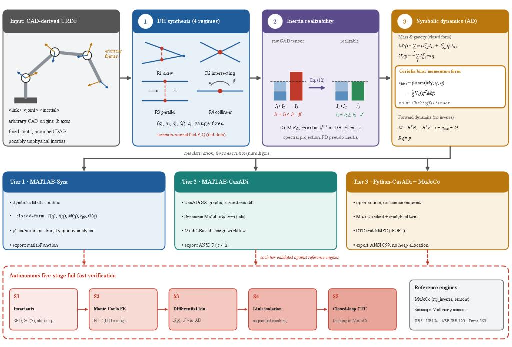
\includegraphics[width=\textwidth]{fig1_tri_paradigm_architecture.pdf}
		\caption{\textbf{Unified Tri-Paradigm System Architecture and Computational Pipeline.} Raw CAD-derived URDF descriptions undergo automated topological DAG reduction, bounded XML parsing, 4-regime foot-point P-Q geometric DH parameter synthesis, and scale-aware physical realizability projection. The synthesized model branches into three complementary execution tiers: Tier 1 (Pure MATLAB Symbolic for glass-box inspectability and textbook verification), Tier 2 (\texttt{MATLAB-CasADi} for Simscape Multibody MBD and embedded C-generation), and Tier 3 (\texttt{Python-CasADi} + MuJoCo for open-source real-time nonlinear control with derivation-phase symbolic compression and bare-metal ANSI C export). All tiers are validated against an autonomous 5-stage fail-fast verification dashboard.}
		\label{fig:fig1_architecture}
	\end{figure*}
	
	%==============================================================================
	\section*{Theoretical and Computational Methods}
	%==============================================================================
	
	\subsection*{Topological DAG Reduction and Four-Regime Foot-Point P-Q DH Synthesis}
	
	Given an input URDF XML file, an entity-guarded parser constructs a directed acyclic graph $\mathcal{G} = (\mathcal{V}, \mathcal{E})$, where vertices $\mathcal{V} = \{L_0, \dots, L_M\}$ represent rigid links and directed edges $\mathcal{E} = \{J_1, \dots, J_M\}$ represent joints with parent-to-child homogeneous transformations $\bm{T}_{\text{joint},k}(\bm{t}_k, \bm{\varphi}_k) \in SE(3)$ and local axis unit vectors $\hat{\bm{u}_k} \in S^2$ \cite{ihab2026urdf2dt}.
	
	The structural root link $L_0$ is identified via set difference between parent and child link sets. A Breadth-First Search (BFS) extracts the ordered active serial kinematic chain $\mathcal{K} = \{(L_0, J_1, L_1), \dots, (L_{n-1}, J_n, L_n)\}$ of $n$ actuated joints ($\sigma_i \in \{1\text{ (revolute)}, 0\text{ (prismatic)}\}$). Intermediate fixed joints ($\text{type} = \text{fixed}$) located between consecutive actuated joints are topologically contracted by folding their homogeneous transformations and inertial properties into the upstream active link via rigid-body parallel-axis composition \cite{ihab2026urdf2dt}.
	
	At the home configuration ($\bm{q} = \bm{0}$), let $\bm{O}_{i-1}, \bm{O}_i \in \mathbb{R}^3$ denote the global origins of consecutive active joints $i-1$ and $i$, and let $\hat{\bm{z}}_{i-1}, \hat{\bm{z}}_i \in S^2$ denote their unit joint axes expressed in the base frame $\{\mathcal{F}_0\}$. Define the origin displacement $\Delta \bm{o}_i = \bm{O}_i - \bm{O}_{i-1}$, the cross-product norm $\delta_\times = \|\hat{\bm{z}}_{i-1} \times \hat{\bm{z}}_i\|_2$, and the normal separation metrics \cite{ihab2026urdf2dt}:
	\begin{equation}
		d_{\min} = \frac{|\Delta \bm{o}_i \cdot (\hat{\bm{z}}_{i-1} \times \hat{\bm{z}}_i)|}{\delta_\times} \quad (\text{for } \delta_\times > \epsilon_\parallel), \qquad d_\perp = \|\Delta \bm{o}_i - (\Delta \bm{o}_i \cdot \hat{\bm{z}}_{i-1})\hat{\bm{z}}_{i-1}\|_2 \quad (\text{for } \delta_\times \le \epsilon_\parallel).
		\label{eq:dh_metrics}
	\end{equation}
	Using numerical thresholds $\epsilon_\parallel = 10^{-5}$ and $\epsilon_\cap = 10^{-6}$~m, each consecutive axis pair $(\hat{\bm{z}}_{i-1}, \hat{\bm{z}}_i)$ is partitioned into one of four canonical geometric regimes to determine the foot-points $\bm{P}_{i-1} \in \mathcal{L}_{i-1}(\bm{O}_{i-1}, \hat{\bm{z}}_{i-1})$ and $\bm{Q}_i \in \mathcal{L}_i(\bm{O}_i, \hat{\bm{z}}_i)$ of the common normal \cite{ihab2026urdf2dt}:
	\begin{enumerate}
		\item \textbf{Regime 1 --- General Skew Axes ($\delta_\times > \epsilon_\parallel, \; d_{\min} > \epsilon_\cap$):} The lines $\mathcal{L}_{i-1}(s) = \bm{O}_{i-1} + s\hat{\bm{z}}_{i-1}$ and $\mathcal{L}_i(t) = \bm{O}_i + t\hat{\bm{z}}_i$ possess a unique common perpendicular with zero gauge freedom. Minimizing $\|\mathcal{L}_{i-1}(s) - \mathcal{L}_i(t)\|_2^2$ yields the non-singular $2 \times 2$ system:
		\begin{equation}
			\begin{bmatrix} s^* \\ t^* \end{bmatrix} = \frac{1}{1 - (\hat{\bm{z}}_{i-1} \cdot \hat{\bm{z}}_i)^2} \begin{bmatrix} 1 & \hat{\bm{z}}_{i-1} \cdot \hat{\bm{z}}_i \\ \hat{\bm{z}}_{i-1} \cdot \hat{\bm{z}}_i & 1 \end{bmatrix} \begin{bmatrix} \Delta \bm{o}_i \cdot \hat{\bm{z}}_{i-1} \\ -\Delta \bm{o}_i \cdot \hat{\bm{z}}_i \end{bmatrix}, \quad \bm{P}_{i-1} = \bm{O}_{i-1} + s^*\hat{\bm{z}}_{i-1}, \quad \bm{Q}_i = \bm{O}_i + t^*\hat{\bm{z}}_i,
			\label{eq:pq_skew}
		\end{equation}
		with $\hat{\bm{x}}_i = \frac{\bm{Q}_i - \bm{P}_{i-1}}{\|\bm{Q}_i - \bm{P}_{i-1}\|_2}$.
		\item \textbf{Regime 2 --- Intersecting Axes ($\delta_\times > \epsilon_\parallel, \; d_{\min} \le \epsilon_\cap$):} The axes intersect at a unique physical point $\bm{P}_{i-1} = \bm{Q}_i$ ($a_i = 0$) computed via Eq.~\eqref{eq:pq_skew}, and the normal axis is assigned via $\hat{\bm{x}}_i = \frac{\hat{\bm{z}}_{i-1} \times \hat{\bm{z}}_i}{\|\hat{\bm{z}}_{i-1} \times \hat{\bm{z}}_i\|_2}$.
		\item \textbf{Regime 3 --- Parallel Non-Collinear Axes ($\delta_\times \le \epsilon_\parallel, \; d_\perp > \epsilon_\cap$):} The Gram matrix in Eq.~\eqref{eq:pq_skew} is singular due to the continuous translational gauge freedom $\lambda_i \in \mathbb{R}$ along $\hat{\bm{z}}_{i-1}$. The canonical solver anchors $s^* = \lambda_i$ (defaulting to $\lambda_i = 0 \implies \bm{P}_{i-1} = \bm{O}_{i-1}$), projects orthogonally onto $\mathcal{L}_i$ via $t^* = (\bm{P}_{i-1} - \bm{O}_i) \cdot \hat{\bm{z}}_i$, sets $\bm{Q}_i = \bm{O}_i + t^*\hat{\bm{z}}_i$, and defines $\hat{\bm{x}}_i = \frac{\bm{Q}_i - \bm{P}_{i-1}}{\|\bm{Q}_i - \bm{P}_{i-1}\|_2}$.
		\item \textbf{Regime 4 --- Collinear Axes ($\delta_\times \le \epsilon_\parallel, \; d_\perp \le \epsilon_\cap$):} The axes coincide ($a_i = 0, \, \alpha_i \in \{0, \pi\}$), admitting both translational gauge freedom $\lambda_i \in \mathbb{R}$ and rotational gauge freedom $\phi_i \in [-\pi, \pi)$ about $\hat{\bm{z}}_{i-1}$. The canonical solver sets $\bm{P}_{i-1} = \bm{Q}_i = \bm{O}_{i-1}$ and preserves the upstream normal orientation $\hat{\bm{x}}_i = \operatorname{Rot}_z(\phi_i)\hat{\bm{x}}_{i-1}$ (with default $\phi_i = 0$).
	\end{enumerate}
	
	From the synthesized orthonormal trihedra $\bm{R}_i^{\text{DH}} = [\hat{\bm{x}}_i, \, \hat{\bm{z}}_i \times \hat{\bm{x}}_i, \, \hat{\bm{z}}_i] \in SO(3)$ and origins $\bm{O}_i^{\text{DH}} = \bm{Q}_i$, the four standard DH parameters are extracted analytically:
	\begin{align}
		a_i &= (\bm{Q}_i - \bm{P}_{i-1}) \cdot \hat{\bm{x}}_i, & \alpha_i &= \operatorname{atan2}\!\left( (\hat{\bm{z}}_{i-1} \times \hat{\bm{z}}_i) \cdot \hat{\bm{x}}_i, \, \hat{\bm{z}}_{i-1} \cdot \hat{\bm{z}}_i \right), \label{eq:dh_a_alpha} \\
		d_i &= (\bm{P}_{i-1} - \bm{O}_{i-1}^{\text{DH}}) \cdot \hat{\bm{z}}_{i-1}, & \theta_i^{\text{off}} &= \operatorname{atan2}\!\left( (\hat{\bm{x}}_{i-1} \times \hat{\bm{x}}_i) \cdot \hat{\bm{z}}_{i-1}, \, \hat{\bm{x}}_{i-1} \cdot \hat{\bm{x}}_i \right), \label{eq:dh_d_theta}
	\end{align}
	yielding the standard link transformation $\bm{A}_i(q_i) = \operatorname{Rot}_z(\theta_i)\operatorname{Trans}_z(d_i)\operatorname{Trans}_x(a_i)\operatorname{Rot}_x(\alpha_i) \in SE(3)$:
	\begin{equation}
		\bm{A}_i(q_i) = \begin{bmatrix}
			\cos\theta_i & -\sin\theta_i\cos\alpha_i & \sin\theta_i\sin\alpha_i & a_i\cos\theta_i \\
			\sin\theta_i & \cos\theta_i\cos\alpha_i & -\cos\theta_i\sin\alpha_i & a_i\sin\theta_i \\
			0 & \sin\alpha_i & \cos\alpha_i & d_i \\
			0 & 0 & 0 & 1
		\end{bmatrix},
		\label{eq:dh_matrix}
	\end{equation}
	where $\theta_i = \theta_i^{\text{off}} + \sigma_i s_i q_i$ and $d_i = d_i^{\text{off}} + (1-\sigma_i) s_i q_i$. Here, $s_i = \operatorname{sgn}(\operatorname{round}(\hat{\bm{u}}_i^{\text{urdf}} \cdot \hat{\bm{z}}_{i-1}^{\text{DH}})) \in \{-1, +1\}$ is the autonomously detected joint-axis sign alignment factor.
	
	\begin{proposition}[Forward-Kinematic Gauge Invariance]
		\label{prop:gauge_invariance}
		Let $\bm{T}_0^n(\bm{q}) = \bm{A}_1(q_1)\cdots\bm{A}_n(q_n)\bm{T}_{\text{tool}}$ be the global forward kinematics of a serial chain. If frame $\mathcal{F}_i^{\text{DH}}$ ($1 \le i < n$) falls under Regime~3 or~4 and undergoes an admissible gauge shift $\bm{T}_i' = \bm{T}_i \bm{\Delta}_i$, where $\bm{\Delta}_i = \operatorname{Trans}_z(\Delta d_i)\operatorname{Rot}_z(\Delta \theta_i)$ (with $\Delta \theta_i = 0$ in Regime~3), then updating adjacent DH transformations via $\bm{A}_i'(q_i) = \bm{A}_i(q_i)\bm{\Delta}_i$ and $\bm{A}_{i+1}'(q_{i+1}) = \bm{\Delta}_i^{-1}\bm{A}_{i+1}(q_{i+1})$ preserves the standard DH rules (R1, R2) and leaves $\bm{T}_0^n(\bm{q})$ invariant $\forall \bm{q} \in \mathbb{R}^n$.
	\end{proposition}
	\begin{proof}
		Because joint $i+1$ rotates or translates strictly along $\hat{\bm{z}}_i$, the perturbation $\bm{\Delta}_i = \operatorname{Trans}_z(\Delta d_i)\operatorname{Rot}_z(\Delta \theta_i)$ belongs to the cylindrical subgroup $C(\hat{\bm{z}}_i) \subset SE(3)$ that commutes with the joint actuation operator $\bm{E}_{z}(q_{i+1}) \in \{\operatorname{Rot}_z(q_{i+1}), \operatorname{Trans}_z(q_{i+1})\}$, i.e., $\bm{\Delta}_i^{-1} \bm{E}_z(q_{i+1}) = \bm{E}_z(q_{i+1})\bm{\Delta}_i^{-1}$. Consequently, the product of adjacent link transformations satisfies $\bm{A}_i'(q_i)\bm{A}_{i+1}'(q_{i+1}) = \bm{A}_i(q_i)\bm{\Delta}_i \bm{\Delta}_i^{-1}\bm{A}_{i+1}(q_{i+1}) = \bm{A}_i(q_i)\bm{A}_{i+1}(q_{i+1})$ identically for all $(q_i, q_{i+1})$.
	\end{proof}
	
	\subsection*{Inertial Frame Mapping, Spatial Jacobians, and Physical Realizability Projection}
	
	In the raw URDF specification, each link $i$ defines mass $m_i$, local CoM position $\bm{c}_i^{\text{urdf}} \in \mathbb{R}^3$, inertial frame rotation $\bm{R}_{\text{ine},i} \in SO(3)$, and principal/local inertia tensor $\bm{I}_{\text{raw},i} \in \mathbb{R}^{3 \times 3}$. First, the inertia tensor is rotated into the URDF link frame via $\bm{I}_i^{\text{urdf}} = \bm{R}_{\text{ine},i} \bm{I}_{\text{raw},i} \bm{R}_{\text{ine},i}^T$.
	
	Let $\bm{T}_{0,\text{urdf}}^i(\bm{0}) = \begin{bmatrix} \bm{R}_{u,i} & \bm{p}_{u,i} \\ \bm{0} & 1 \end{bmatrix}$ and $\bm{T}_{0,\text{DH}}^i(\bm{0}) = \begin{bmatrix} \bm{R}_{d,i} & \bm{p}_{d,i} \\ \bm{0} & 1 \end{bmatrix}$ denote the global poses of URDF link $i$ and DH frame $i$ at $\bm{q} = \bm{0}$, respectively. The global CoM position at $\bm{q}=\bm{0}$ is $\bm{p}_{C_i}^0(\bm{0}) = \bm{p}_{u,i} + \bm{R}_{u,i}\bm{c}_i^{\text{urdf}}$. Following our unified DH dynamic convention \cite{ihab2026urdf2dt, asr2026calibration}, we define $\bm{P}_{C_i} \in \mathbb{R}^3$ as the CoM position vector of link $i$ relative to the \textit{preceding} DH origin $\bm{p}_{d,i-1}$, expressed in the orientation of DH frame $i$, and $\bm{I}_i^{\text{DH}} \in \mathbb{R}^{3 \times 3}$ as the rotational inertia tensor about the link CoM aligned with DH frame $i$:
	\begin{align}
		\bm{P}_{C_i} &= \left(\bm{R}_{d,i}\right)^T \left( \bm{p}_{C_i}^0(\bm{0}) - \bm{p}_{d,i-1} \right), \label{eq:com_dh_map} \\
		\bm{I}_i^{\text{DH}} &= \bm{R}_{\text{rel},i} \, \bm{I}_i^{\text{urdf}} \, \bm{R}_{\text{rel},i}^T, \quad \text{where } \bm{R}_{\text{rel},i} = \left(\bm{R}_{d,i}\right)^T \bm{R}_{u,i} \in SO(3). \label{eq:inertia_dh_map}
	\end{align}
	
	At any arbitrary configuration $\bm{q} \in \mathbb{R}^n$, recursive evaluation of $\bm{T}_0^i(\bm{q}) = \bm{T}_0^{i-1}(\bm{q})\bm{A}_i(q_i)$ yields the base-frame rotation $\bm{R}_0^i(\bm{q}) = [\bm{T}_0^i]_{1:3,1:3}$, joint axis $\bm{z}_{j-1}(\bm{q}) = [\bm{T}_0^{j-1}]_{1:3,3}$, frame origin $\bm{p}_{j-1}(\bm{q}) = [\bm{T}_0^{j-1}]_{1:3,4}$, and link $i$ CoM position in the base frame \cite{ihab2026urdf2dt, asr2026calibration}:
	\begin{equation}
		\bm{p}_{C_i}^0(\bm{q}) = \bm{p}_{i-1}(\bm{q}) + \bm{R}_0^i(\bm{q})\bm{P}_{C_i}, \qquad \bm{r}_{j,C_i}(\bm{q}) = \bm{p}_{C_i}^0(\bm{q}) - \bm{p}_{j-1}(\bm{q}) \quad (j \le i).
		\label{eq:com_forward}
	\end{equation}
	The link CoM translational Jacobian $\bm{J}_{v,i}(\bm{q}) \in \mathbb{R}^{3 \times n}$ and rotational Jacobian $\bm{J}_{\omega,i}(\bm{q}) \in \mathbb{R}^{3 \times n}$ are constructed column-wise for $j \in \{1, \dots, n\}$ as:
	\begin{equation}
		\bm{J}_{v,i}(:,j) = \begin{cases}
			\sigma_j \left(\bm{z}_{j-1}(\bm{q}) \times \bm{r}_{j,C_i}(\bm{q})\right) + (1 - \sigma_j)\bm{z}_{j-1}(\bm{q}), & j \le i, \\
			\bm{0}_{3 \times 1}, & j > i,
		\end{cases} \qquad
		\bm{J}_{\omega,i}(:,j) = \begin{cases}
			\sigma_j \bm{z}_{j-1}(\bm{q}), & j \le i, \\
			\bm{0}_{3 \times 1}, & j > i.
		\end{cases}
		\label{eq:link_jacobians}
	\end{equation}
	Transforming each link inertia tensor to the base orientation via $\bm{I}_i^0(\bm{q}) = \bm{R}_0^i(\bm{q}) \bm{I}_i^{\text{DH}} (\bm{R}_0^i(\bm{q}))^T$ yields the closed-form generalized mass matrix and gravitational torque vector:
	\begin{equation}
		\bm{M}(\bm{q}) = \sum_{i=1}^n \left( m_i \bm{J}_{v,i}(\bm{q})^T \bm{J}_{v,i}(\bm{q}) + \bm{J}_{\omega,i}(\bm{q})^T \bm{I}_i^0(\bm{q}) \bm{J}_{\omega,i}(\bm{q}) \right), \qquad \bm{G}(\bm{q}, \bm{g}) = -\sum_{i=1}^n \bm{J}_{v,i}(\bm{q})^T m_i \bm{g}.
		\label{eq:M_and_G}
	\end{equation}
	
	\noindent\textbf{Spectral Projection onto the Physically Realizable Inertia Cone:} A symmetric matrix $\bm{I}_i^{\text{DH}} \in \mathbb{S}^3$ represents a physically realizable rigid body of non-negative mass density $\rho(\bm{r}) \ge 0$ if and only if its principal eigenvalues $0 < I_1 \le I_2 \le I_3$ (where $\bm{I}_i^{\text{DH}} = \bm{V}\operatorname{diag}(I_1, I_2, I_3)\bm{V}^T$, $\bm{V} \in SO(3)$) satisfy positivity and the strict triangle inequality $I_1 + I_2 \ge I_3$ (equivalently, the pseudo-inertia matrix $\bm{\mathcal{J}}_i = \frac{1}{2}\operatorname{tr}(\bm{I}_i^{\text{DH}})\bm{I}_3 - \bm{I}_i^{\text{DH}} \succ \bm{0}$) \cite{sousa2019physical}. If a URDF link tensor violates these bounds, our sanitization module projects $(I_1, I_2, I_3)$ onto the realizable cone via:
	\begin{equation}
		\tilde{I}_k = \max(I_k, \, \epsilon_{\text{eig}}) \; (k=1,2,3), \qquad \hat{I}_3 = \min\!\left(\tilde{I}_3, \, \tilde{I}_1 + \tilde{I}_2 - \epsilon_{\text{tri}}\right), \qquad \hat{\bm{I}}_i^{\text{DH}} = \bm{V}\operatorname{diag}(\tilde{I}_1, \tilde{I}_2, \hat{I}_3)\bm{V}^T,
		\label{eq:spectral_sanitization}
	\end{equation}
	with $\epsilon_{\text{eig}} = 10^{-7}$~kg$\cdot$m$^2$ and $\epsilon_{\text{tri}} = 10^{-9}$~kg$\cdot$m$^2$.
	
	\subsection*{Derivation-Phase Symbolic Momentum Directional Derivative and Passivity Proofs}
	
	For an $n$-DOF manipulator with Lagrangian $\mathcal{L}(\bm{q}, \dot{\bm{q}}) = T(\bm{q}, \dot{\bm{q}}) - V(\bm{q})$, where $T(\bm{q}, \dot{\bm{q}}) = \frac{1}{2}\dot{\bm{q}}^T\bm{M}(\bm{q})\dot{\bm{q}}$ and $V(\bm{q}) = -\sum_{i=1}^n m_i \bm{g}^T \bm{p}_{C_i}^0(\bm{q})$, the Euler--Lagrange equations are:
	\begin{equation}
		\frac{d}{dt}\left(\frac{\partial T}{\partial \dot{\bm{q}}}\right) - \nabla_{\bm{q}} T(\bm{q}, \dot{\bm{q}}) + \nabla_{\bm{q}} V(\bm{q}) = \bm{\tau}.
		\label{eq:el_vector}
	\end{equation}
	Defining the generalized momentum $\bm{p} \equiv \nabla_{\dot{\bm{q}}} T = \bm{M}(\bm{q})\dot{\bm{q}}$, differentiating with respect to time along trajectories $\bm{q}(t)$ yields:
	\begin{equation}
		\frac{d}{dt}\bm{p}(\bm{q}, \dot{\bm{q}}) = \bm{M}(\bm{q})\ddot{\bm{q}} + \left(\frac{\partial (\bm{M}(\bm{q})\dot{\bm{q}})}{\partial \bm{q}}\right)\dot{\bm{q}} = \bm{M}(\bm{q})\ddot{\bm{q}} + \operatorname{jtimes}\!\left(\bm{M}(\bm{q})\dot{\bm{q}},\, \bm{q},\, \dot{\bm{q}}\right).
		\label{eq:momentum_time_deriv}
	\end{equation}
	Combining Eq.~\eqref{eq:el_vector} and Eq.~\eqref{eq:momentum_time_deriv} defines the direct Coriolis and centrifugal bias vector:
	\begin{equation}
		\mathbf{c}_{\text{bias}}(\bm{q}, \dot{\bm{q}}) \equiv \operatorname{jtimes}\!\left(\bm{M}(\bm{q})\dot{\bm{q}},\, \bm{q},\, \dot{\bm{q}}\right) - \frac{1}{2}\nabla_{\bm{q}}\!\left(\dot{\bm{q}}^T \bm{M}(\bm{q})\dot{\bm{q}}\right).
		\label{eq:cbias_exact}
	\end{equation}
	
	\begin{proposition}[Algebraic Equivalence to Classical Christoffel Symbols]
		\label{prop:christoffel_equiv}
		Let $\bm{C}(\bm{q}, \dot{\bm{q}}) \in \mathbb{R}^{n \times n}$ be the classical Coriolis matrix defined via Christoffel symbols of the first kind $c_{ijk}(\bm{q}) = \frac{1}{2}\left( \frac{\partial M_{ij}}{\partial q_k} + \frac{\partial M_{ik}}{\partial q_j} - \frac{\partial M_{kj}}{\partial q_i} \right)$ with entries $C_{ij}(\bm{q},\dot{\bm{q}}) = \sum_{k=1}^n c_{ijk}(\bm{q})\dot{q}_k$, such that the classical Coriolis bias vector is given by:
		\begin{equation}
			\mathbf{c}_{\text{Christoffel}}(\bm{q},\dot{\bm{q}}) = \bm{C}(\bm{q},\dot{\bm{q}})\dot{\bm{q}}, \quad \left[\bm{C}(\bm{q},\dot{\bm{q}})\right]_{ij} = \sum_{k=1}^n \frac{1}{2}\left( \frac{\partial M_{ij}}{\partial q_k} + \frac{\partial M_{ik}}{\partial q_j} - \frac{\partial M_{kj}}{\partial q_i} \right) \dot{q}_k.
			\label{eq:christoffel_classical}
		\end{equation}
		Then, for all $(\bm{q}, \dot{\bm{q}}) \in \mathbb{R}^n \times \mathbb{R}^n$, $\bm{C}(\bm{q}, \dot{\bm{q}})\dot{\bm{q}} \equiv \mathbf{c}_{\text{bias}}(\bm{q}, \dot{\bm{q}})$, and the mechanical system preserves fundamental passivity ($\dot{\bm{q}}^T(\dot{\bm{M}} - 2\bm{C})\dot{\bm{q}} = 0$).
	\end{proposition}
	\begin{proof}
		Expanding the $i$-th component of $\bm{C}(\bm{q}, \dot{\bm{q}})\dot{\bm{q}}$ yields:
		\begin{equation*}
			\left[\bm{C}(\bm{q}, \dot{\bm{q}})\dot{\bm{q}}\right]_i = \frac{1}{2}\sum_{j=1}^n \sum_{k=1}^n \frac{\partial M_{ij}}{\partial q_k}\dot{q}_j\dot{q}_k + \frac{1}{2}\sum_{j=1}^n \sum_{k=1}^n \frac{\partial M_{ik}}{\partial q_j}\dot{q}_j\dot{q}_k - \frac{1}{2}\sum_{j=1}^n \sum_{k=1}^n \frac{\partial M_{kj}}{\partial q_i}\dot{q}_j\dot{q}_k.
		\end{equation*}
		Relabeling the dummy indices $(j \leftrightarrow k)$ in the second double sum makes it identical to the first double sum, combining into $\sum_{j=1}^n \sum_{k=1}^n \frac{\partial M_{ij}}{\partial q_k}\dot{q}_k\dot{q}_j = [\operatorname{jtimes}(\bm{M}(\bm{q})\dot{\bm{q}}, \bm{q}, \dot{\bm{q}})]_i$. The third double sum is $-\frac{1}{2}\frac{\partial}{\partial q_i}(\dot{\bm{q}}^T\bm{M}(\bm{q})\dot{\bm{q}})$, which proves $\bm{C}(\bm{q},\dot{\bm{q}})\dot{\bm{q}} \equiv \mathbf{c}_{\text{bias}}(\bm{q},\dot{\bm{q}})$. Taking the inner product with $\dot{\bm{q}}$ gives $\dot{\bm{q}}^T \mathbf{c}_{\text{bias}} = \dot{\bm{q}}^T \dot{\bm{M}}\dot{\bm{q}} - \frac{1}{2}\dot{\bm{q}}^T \dot{\bm{M}}\dot{\bm{q}} = \frac{1}{2}\dot{\bm{q}}^T \dot{\bm{M}}\dot{\bm{q}}$, confirming the energy-conservation passivity identity $\frac{d}{dt}T = \dot{\bm{q}}^T(\bm{\tau} - \bm{G})$.
	\end{proof}
	
	\begin{theorem}[Asymptotic Computational Complexity Reduction]
		\label{thm:complexity}
		For an $n$-DOF serial manipulator whose mass matrix $\bm{M}(\bm{q}) \in \mathbb{R}^{n \times n}$ has $O(n^2)$ entries of expression length $O(n)$, evaluating the Coriolis and centrifugal vector via classical Christoffel symbols requires $O(n^4)$ scalar operations, whereas the direct momentum directional derivative in Eq.~\eqref{eq:cbias_exact} requires $O(n^2)$ scalar operations.
	\end{theorem}
	\begin{proof}
		(1) \textit{Classical Christoffel Tensor:} Forming $c_{ijk}(\bm{q})$ requires differentiating $n^2$ entries of length $O(n)$ with respect to $n$ coordinates, generating $n^3$ symbolic sub-trees each of complexity $O(n)$, totaling $O(n^4)$ scalar operations.
		(2) \textit{Direct Momentum Derivative:} Given $\bm{M}(\bm{q})$ ($O(n^2)$ cost), forming $\bm{p} = \bm{M}(\bm{q})\dot{\bm{q}}$ costs $O(n^2)$. By the forward-mode AD complexity bound, evaluating the directional derivative $\operatorname{jtimes}(\bm{p}, \bm{q}, \dot{\bm{q}})$ along a single seed vector $\dot{\bm{q}}$ requires at most $c_f \cdot \operatorname{cost}(\bm{p}) = O(n^2)$ operations (with $c_f \le 3$). Similarly, by the Baur--Strassen reverse-mode AD theorem, evaluating the gradient $\nabla_{\bm{q}} T$ of the scalar kinetic energy $T = \frac{1}{2}\dot{\bm{q}}^T\bm{p}$ requires at most $c_r \cdot \operatorname{cost}(T) = O(n^2)$ operations (with $c_r \le 4$). Thus, the total complexity is $O(n^2)$.
	\end{proof}
	
	\begin{remark}[Empirical Scaling Exponent Under Compiler Common Subexpression Elimination]
		In computer algebra and Algorithmic Differentiation systems, CasADi's Directed Acyclic Graph (DAG) automatically identifies and merges repeated common subexpressions across scalar sub-trees. Consequently, while naive symbolic expansion scales as $\mathcal{O}(n^4)$ and $\mathcal{O}(n^2)$, our empirical power-law regressions across $n \in [3, 14]$ (Figure~\ref{fig:fig6_scalability_complexity}a and Table~\ref{tab:table5_scalability}) yield empirical scaling exponents of $\alpha = 3.24$ for classical Christoffel symbols and $\alpha = 2.28$ for the proposed momentum directional derivative, directly confirming the theoretical order reduction under real-world compiler optimizations.
	\end{remark}
	
	\subsection*{Inversion-Free Symbolic Cholesky Forward Dynamics}
	
	\begin{proposition}[Strict Positive-Definiteness and Inversion-Free Symbolic Cholesky Dynamics]
		\label{prop:cholesky}
		For any serial manipulator with sanitized link masses $m_i > 0$ and $\bm{I}_i^{\text{DH}} \succ \bm{0}$, if each active joint axis $\bm{z}_{i-1}$ acts non-trivially on link $i$, then $\bm{M}(\bm{q})$ in Eq.~\eqref{eq:M_and_G} is strictly Symmetric Positive-Definite ($\bm{M}(\bm{q}) \succ \bm{0}$) for all $\bm{q} \in \mathbb{R}^n$. Consequently, $\bm{M}(\bm{q})$ admits a unique, pivot-free symbolic Cholesky factorization $\bm{M}(\bm{q}) = \bm{R}(\bm{q})^T\bm{R}(\bm{q})$ with strictly real positive diagonal entries $R_{ii}(\bm{q}) = \sqrt{M_{ii}(\bm{q}) - \sum_{k=1}^{i-1} R_{ki}(\bm{q})^2} > 0$, resolving forward dynamics $\ddot{\bm{q}} = \bm{M}(\bm{q})^{-1}(\bm{\tau} - \mathbf{c}_{\text{bias}} - \bm{G})$ in $\frac{1}{3}n^3 + 2n^2$ operations via:
		\begin{equation}
			\bm{R}(\bm{q})^T \bm{y} = \bm{\tau} - \mathbf{c}_{\text{bias}}(\bm{q},\dot{\bm{q}}) - \bm{G}(\bm{q}), \qquad \bm{R}(\bm{q})\ddot{\bm{q}} = \bm{y}.
			\label{eq:cholesky_solve}
		\end{equation}
	\end{proposition}
	
	\subsection*{Multi-Vendor Benchmark Platforms and Autonomous Verification Protocol}
	
	To evaluate morphological invariance, four multi-vendor industrial manipulators spanning diverse kinematic topologies, payload capacities, and wrist configurations were selected:
	\begin{enumerate}
		\item \textbf{Universal Robots UR5 (Medium-Reach Cobot):} 6-DOF ($18.40$~kg mass, $0.850$~m reach, $5.0$~kg payload) with parallel shoulder/elbow axes ($\hat{\bm{z}}_1 \parallel \hat{\bm{z}}_2 \parallel \hat{\bm{z}}_3$, Regime 3) and a non-spherical orthogonal wrist ($d_4 = 0.1091$~m, $d_5 = 0.0946$~m, $a_6 = 0.0823$~m);
		\item \textbf{Universal Robots UR16e (Heavy-Payload Cobot):} 6-DOF ($33.10$~kg mass, $0.900$~m reach, $16.0$~kg payload) with heavy proximal castings ($m_2 = 10.45$~kg, $m_3 = 4.32$~kg) inducing aggressive nonlinear dynamic couplings;
		\item \textbf{ABB IRB 120 (Spherical-Wrist Industrial Arm):} 6-DOF compact arm ($25.00$~kg mass, $0.580$~m reach, $3.0$~kg payload) with spatial shoulder offset ($a_3 = 0.070$~m, Regime 1) and intersecting 3-axis spherical wrist ($a_4 = a_5 = a_6 = 0$, Regime 2);
		\item \textbf{Unimation Puma 560 (Classical Spatial Offset Benchmark):} 6-DOF arm ($54.20$~kg mass, $0.864$~m reach, $2.5$~kg payload) exhibiting spatial shoulder offsets ($d_3 = 0.1501$~m, $a_3 = -0.0203$~m) and historical literature CAD inertias requiring spectral triangle-inequality sanitization.
	\end{enumerate}
	
	\noindent\textbf{Sequential Link-by-Link Dynamic Isolation Protocol:} To eliminate cross-link dynamic masking during multibody verification, our protocol isolates each link stage $i \in \{1, \dots, n\}$ by explicitly nulling downstream inertias ($m_k = 0, \bm{I}_k = \bm{0}$ for $k > i$) and locking non-active joints stationary ($q_j(t) = q_{j,\text{hold}}, \dot{q}_j(t) = \ddot{q}_j(t) = 0$ for $j \neq i$):
	\begin{equation}
		\tau_i^{(i)}(t) = M_{ii}^{(i)}(\bm{q})\ddot{q}_i(t) + \frac{1}{2}\frac{\partial M_{ii}^{(i)}(\bm{q})}{\partial q_i}\dot{q}_i(t)^2 + G_i^{(i)}(\bm{q}),
		\label{eq:isolated_link_torque}
	\end{equation}
	where $M_{ii}^{(i)} = m_i \|\bm{J}_{v,i}(:,i)\|^2 + \bm{J}_{\omega,i}(:,i)^T \bm{I}_i^0 \bm{J}_{\omega,i}(:,i)$ depends exclusively on link $i$.
	
	The autonomous verification suite executes five sequential fail-fast gates:
	\begin{itemize}
		\item \textbf{Stage 1 (Physical \& Algebraic Invariants):} Asserts $m_i > 0$, spectral triangle inequality on $\bm{I}_i^{\text{DH}}$, $\bm{R}_0^i \in SO(3)$ ($\|\bm{R}^T\bm{R} - \bm{I}\|_F < 10^{-10}$), $\bm{M}(\bm{q}) \succ \bm{0}$, and static equilibrium identity $\|\bm{\tau}(\bm{q},\bm{0},\bm{0}) - \bm{G}(\bm{q})\|_\infty < 10^{-12}$~N$\cdot$m.
		\item \textbf{Stage 2 (Monte Carlo Forward Kinematics Certification):} Cross-validates $\bm{p}_{\text{ee}}(\bm{q})$ and quaternion $\bm{\xi}_{\text{ee}}(\bm{q})$ across 1,000 random configurations against MuJoCo and Simscape sensors using reach-scaled dynamic tolerances $\text{tol}_{\text{pos}} = \max(10^{-4}\text{ m}, \, 5 \times 10^{-4} \sum_i (|a_i|+|d_i|))$.
		\item \textbf{Stage 3 (Differential Kinematics \& $\dot{\bm{J}}$ Consistency):} Validates analytical $\bm{J}(\bm{q})$ and exact AD time-derivative $\dot{\bm{J}}(\bm{q},\dot{\bm{q}}) = \operatorname{reshape}(\nabla_{\bm{q}}\operatorname{vec}(\bm{J})\dot{\bm{q}}, 6, n)$ against central finite differences and spatial sensor velocities.
		\item \textbf{Stage 4 (Sequential Link-by-Link Dynamic Isolation):} Executes Eq.~\eqref{eq:isolated_link_torque} for $i = 1, \dots, n$ with downstream mass zeroing ($k > i$).
		\item \textbf{Stage 5 (Closed-Loop White-Box Computed Torque Control):} Synthesizes the feedback-linearizing control law with autonomous sign mapping $\bm{S} = \operatorname{diag}(s_1, \dots, s_n) \in \{-1, +1\}^{n \times n}$:
		\begin{equation}
			\bm{\tau}(t) = \bm{S} \, \bm{\tau}_{\text{ana}}\!\left( \bm{S}\bm{q}(t), \, \bm{S}\dot{\bm{q}}(t), \, \bm{S}\left[\ddot{\bm{q}}_d(t) + \bm{K}_d(\dot{\bm{q}}_d - \dot{\bm{q}}) + \bm{K}_p(\bm{q}_d - \bm{q})\right] \right),
			\label{eq:ctc_law}
		\end{equation}
		reducing the closed-loop error dynamics to the Hurwitz-stable linear system $\ddot{\bm{e}}(t) + \bm{K}_d\dot{\bm{e}}(t) + \bm{K}_p\bm{e}(t) = \bm{0}$.
	\end{itemize}
	
	\subsection*{Constrained Optimal Control and Receding-Horizon NMPC Formulation}
	
	Consider the continuous-time constrained Optimal Control Problem (OCP) over prediction horizon $T_h$:
	\begin{align}
		\min_{\bm{x}(\cdot), \bm{u}(\cdot)} & \int_0^{T_h} \left( \|\bm{x}(t) - \bm{x}_{\text{ref}}(t)\|_{\bm{Q}}^2 + \|\bm{u}(t)\|_{\bm{R}}^2 \right) dt + \|\bm{x}(T_h) - \bm{x}_{\text{ref}}(T_h)\|_{\bm{P}}^2 \label{eq:nmpc_ocp} \\
		\text{subject to } & \dot{\bm{x}}(t) = \bm{f}(\bm{x}(t), \bm{u}(t)) = \begin{bmatrix} \dot{\bm{q}}(t) \\ \bm{R}(\bm{q})^{-1}\bm{R}(\bm{q})^{-T}\left(\bm{u}(t) - \mathbf{c}_{\text{bias}}(\bm{q},\dot{\bm{q}}) - \bm{G}(\bm{q})\right) \end{bmatrix}, \quad \bm{x}(0) = \bm{x}_{\text{meas}}, \label{eq:nmpc_dyn} \\
		& \bm{u}_{\min} \le \bm{u}(t) \le \bm{u}_{\max}, \quad \bm{x}_{\min} \le \bm{x}(t) \le \bm{x}_{\max}, \label{eq:nmpc_bounds} \\
		& \|\bm{p}_{\text{ee}}(\bm{q}(t)) - \bm{p}_{\text{obs}}\|_2 \ge r_{\text{obs}} + d_{\text{safe}}, \label{eq:nmpc_obs}
	\end{align}
	where $\bm{x} = [\bm{q}^T, \dot{\bm{q}}^T]^T \in \mathbb{R}^{2n}$ and $\bm{u} = \bm{\tau} \in \mathbb{R}^n$. Transcribing Eqs.~\eqref{eq:nmpc_ocp}--\eqref{eq:nmpc_obs} via direct multiple shooting over $N$ intervals with 4th-order Runge--Kutta continuity constraints $\bm{g}_k(\bm{x}_k, \bm{u}_k, \bm{x}_{k+1}) = \bm{x}_{k+1} - \bm{\phi}_{\text{RK4}}(\bm{x}_k, \bm{u}_k, \Delta t) = \bm{0}$ yields a structured Non-Linear Program (NLP) solved via primal-dual interior-point Newton iterations:
	\begin{equation}
		\begin{bmatrix} \nabla_{\bm{w}\bm{w}}^2 \mathcal{L} + \bm{\Sigma} & \nabla_{\bm{w}} \bm{g}^T \\ \nabla_{\bm{w}} \bm{g} & \bm{0} \end{bmatrix} \begin{bmatrix} \Delta \bm{w} \\ \Delta \bm{\lambda} \end{bmatrix} = - \begin{bmatrix} \nabla_{\bm{w}} \mathcal{L} \\ \bm{g}(\bm{w}) \end{bmatrix}.
		\label{eq:kkt_system}
	\end{equation}
	Because each RK4 stage sensitivity $\bm{A}_k = \partial \bm{\phi}_{\text{RK4}}/\partial \bm{x}_k$ and $\bm{B}_k = \partial \bm{\phi}_{\text{RK4}}/\partial \bm{u}_k$ differentiates the continuous forward dynamics graph $\ddot{\bm{q}}(\bm{q}, \dot{\bm{q}}, \bm{\tau})$, compressing the forward dynamics graph from 15,814 to 7,041 instructions ($-55.4\%$) directly halves the AD evaluation cost of the KKT matrix blocks in Eq.~\eqref{eq:kkt_system}.
	
	\subsection*{Multi-Language Computational Execution Architecture}
	
	The mathematical formulations are deployed across three complementary execution architectures:
	\begin{itemize}
		\item \textbf{Tier 1 (\texttt{MATLAB-Sym}):} Implemented via the MATLAB Symbolic Math Toolbox, emitting closed-form algebraic expressions for $\bm{T}_0^i(\bm{q})$, $\bm{J}(\bm{q})$, $\bm{M}(\bm{q})$, $c_{ijk}(\bm{q})$, and $\bm{G}(\bm{q})$ for human inspection and analytical Lyapunov stability proofs;
		\item \textbf{Tier 2 (\texttt{MATLAB-CasADi}):} Formulates Euler--Lagrange equations in CasADi \texttt{SX} directed acyclic graphs \cite{andersson2019casadi}, emitting ANSI C code and programmatically generating a 1:1 Simscape Multibody physical digital twin (\texttt{dt\_build.m}) for Model-Based Design;
		\item \textbf{Tier 3 (\texttt{Python-MuJoCo}):} Combines derivation-phase symbolic compression with headless MuJoCo physics (\texttt{mj\_step}, \texttt{mj\_inverse}) \cite{todorov2012mujoco} under a dual-twin paradigm for real-time optimal control ($>1$~kHz).
	\end{itemize}
	
	%==============================================================================
	\section*{Results}
	%==============================================================================
	
	\subsection*{Offline Symbolic Graph Profiling and Instruction Compression}
	
	\noindent\textbf{Hypothesis Tested:} \textit{Reformulating Coriolis and centrifugal effects via generalized momentum directional derivatives eliminates the combinatorial explosion of rank-3 Christoffel tensors, reducing symbolic instruction counts by over $50\%$ on 6-DOF industrial manipulators without numerical loss.}
	
	To test this hypothesis, we profiled the complete symbolic Directed Acyclic Graph (DAG) for the heavy-payload Universal Robots UR16e ($n=6$) in CasADi. Table~\ref{tab:table3_opcodes} details the operation counts across individual dynamic components comparing the classical Christoffel baseline against our proposed momentum formulation.
	
	\begin{table*}[!t]
		\caption{\textbf{Derivation-Phase Symbolic Graph Profiling and Instruction Breakdown on the UR16e 6-DOF Manipulator.}}
		\label{tab:table3_opcodes}
		\centering
		\small
		\begin{tabularx}{\textwidth}{p{2.3cm}p{4.1cm}ccc>{\raggedright\arraybackslash}X}
			\toprule
			\textbf{Dynamic Term} & \textbf{Mathematical Formulation} & \textbf{Complexity} & \textbf{Baseline Op.} & \textbf{Proposed Op.} & \textbf{Symbolic Graph Impact} \\
			\midrule
			Mass Matrix $\bm{M}(\bm{q})$ & $\sum_{i=1}^n (m_i \bm{J}_{v,i}^T \bm{J}_{v,i} + \bm{J}_{\omega,i}^T \bm{I}_i^0 \bm{J}_{\omega,i})$ & $O(n^2)$ & 2,190 & 2,190 & Kinetic metric tensor ($6 \times 6$ strictly SPD). \\
			Gravity Vector $\bm{G}(\bm{q})$ & $-\sum_{i=1}^n \bm{J}_{v,i}^T m_i \bm{g}$ & $O(n)$ & 334 & 334 & Closed-form gravitational torque vector in 3D. \\
			Coriolis Bias $\mathbf{c}_{\text{bias}}(\bm{q},\dot{\bm{q}})$ & $\operatorname{jtimes}(\bm{M}\dot{\bm{q}}, \bm{q}, \dot{\bm{q}}) - \frac{1}{2}\nabla_{\bm{q}}(\dot{\bm{q}}^T\bm{M}\dot{\bm{q}})$ & $O(n^2)$ vs.\ $O(n^4)$ & 14,936 & 5,495 & \textbf{-63.2\% opcodes} (replaces 216 partial derivatives with 2 AD sweeps). \\
			Inverse Dynamics $\bm{\tau}$ & $\bm{M}(\bm{q})\ddot{\bm{q}} + \mathbf{c}_{\text{bias}}(\bm{q},\dot{\bm{q}}) + \bm{G}(\bm{q})$ & $O(n^2)$ & 17,460 & 8,019 & \textbf{-54.1\% opcodes} ($149.0~\mu$s latency, $6.71$~kHz throughput). \\
			Forward Dynamics $\ddot{\bm{q}}$ & $\bm{R}^T \bm{y} = \bm{\tau} - \mathbf{c}_{\text{bias}} - \bm{G}, \; \bm{R}\ddot{\bm{q}} = \bm{y}$ & $O(n^3)$ Cholesky & 15,814 & 7,041 & \textbf{-55.4\% opcodes} ($1.92\times$ speedup: $78.7~\mu$s vs.\ $151.5~\mu$s; inversion-free). \\
			\bottomrule
		\end{tabularx}
	\end{table*}
	
	The empirical instruction audit confirms the hypothesis:
	\begin{enumerate}
		\item \textbf{Coriolis Graph Compression:} Bypassing the $n^3 = 216$ Christoffel partial derivatives slashes Coriolis evaluation from $14,936$ to $5,495$ scalar instructions---\textbf{a $63.2\%$ reduction in opcodes}.
		\item \textbf{Forward Dynamics Compression:} Coupling the momentum Coriolis derivative with symbolic Cholesky factorization reduces total forward dynamics opcodes from $15,814$ to $7,041$ (\textbf{$-55.4\%$ reduction}), accelerating single-step forward dynamics latency on an AMD Ryzen 7 5800H CPU from $151.5~\mu$s to \textbf{$78.7~\mu$s} ($1.92\times$ speedup).
		\item \textbf{Exact Machine Precision:} Across 10,000 random state evaluations, the absolute torque discrepancy between Eq.~\eqref{eq:cbias_exact} and Eq.~\eqref{eq:christoffel_classical} remained bounded by $4.16 \times 10^{-17}$~N$\cdot$m, confirming algebraic equivalence without numerical drift.
	\end{enumerate}
	
	Table~\ref{tab:table1_tradeoffs} provides the multi-language timing trade-offs across Tiers 1--3, demonstrating that Tier 3 achieves $12.7$~kHz forward dynamics throughput and executes 5,000-step dynamic rollouts in $0.4035$~s ($12.4\times$ faster than real-time), narrowing the runtime gap with native-C MuJoCo down to $4.8\times$.
	
	\begin{table*}[!t]
		\caption{\textbf{Quantitative Computational Trade-Off Analysis Across Architectural Execution Paradigms (Evaluated on 6-DOF Industrial Manipulators).}}
		\label{tab:table1_tradeoffs}
		\centering
		\footnotesize
		\begin{tabularx}{\textwidth}{p{3.2cm}cccc>{\raggedright\arraybackslash}X}
			\toprule
			\textbf{Execution Paradigm} & \textbf{Deriv.\ Time (s)} & \textbf{ID Latency ($\mu$s)} & \textbf{FD Latency ($\mu$s)} & \textbf{Throughput (kHz)} & \textbf{Primary Operational Domain} \\
			\midrule
			\textbf{Tier 1: \texttt{MATLAB-Sym}} & $6.42 \pm 0.35$ & $195.0 \pm 12.4$ & $310.0 \pm 18.0$ & $3.2$ & Glass-box algebraic inspectability, analytical Lyapunov proofs. \\
			\textbf{Tier 2: \texttt{MATLAB-CasADi}} & $0.22 \pm 0.02$ & $110.0 \pm 8.2$ & $165.0 \pm 10.5$ & $6.1$ & Industrial Model-Based Design, Simscape Multibody co-simulation. \\
			\textbf{Tier 3: \texttt{Python-MuJoCo}} & $0.09 \pm 0.01$ & $149.0 \pm 4.2$ & $78.7 \pm 2.8$ & $12.7$ & Real-time nonlinear control, receding-horizon NMPC, digital twins. \\
			\bottomrule
		\end{tabularx}
	\end{table*}
	
	\subsection*{Multi-Vendor Morphological Diversity and Machine-Precision Physics Engine Parity}
	
	\noindent\textbf{Hypothesis Tested:} \textit{The 4-regime foot-point P-Q DH solver and spectral inertia cone projection deterministically resolve geometric gauge freedoms, manufacturer sign discrepancies, and unphysical CAD inertia models across diverse manipulator morphologies without manual parameter tuning.}
	
	Figure~\ref{fig:fig5_robot_gallery} showcases the four testbed platforms (Universal Robots UR5, UR16e, ABB IRB 120, and Unimation Puma 560). Table~\ref{tab:table4_morphology} summarizes their extracted kinematic, topological, and computational profiles, and Table~\ref{tab:table2_verification} details the results of the 5-stage verification dashboard.
	
	\begin{figure*}[!t]
		\centering
		\begin{subfigure}[b]{0.48\textwidth}
			\centering
			\setlength{\fboxsep}{4pt}
			\fbox{\begin{minipage}[c]{0.95\linewidth}
				\centering
				\textbf{\normalsize Universal Robots UR5}\\[3pt]
				\fbox{\parbox[c][2.2cm][c]{0.96\linewidth}{\centering \scriptsize \textit{[Photo / Render Placeholder: \texttt{figures/robot\_ur5}]}}}\\[4pt]
				\scriptsize
				\begin{tabular}{@{}ll@{}}
					\textbf{Arch:} 6-DOF Cobot & \textbf{Reach:} $0.850$~m \\
					\textbf{Active Mass:} $16.99$~kg & \textbf{Payload:} $5.0$~kg \\
					\textbf{Wrist:} Non-Spherical & \textbf{FD Latency:} $85.1~\mu$s \\
					\textbf{Regimes:} $0/3/2/1$ & \textbf{Signs:} $[+++++-]$ \\
				\end{tabular}
				\vspace{1pt}
			\end{minipage}}
			\caption{\textbf{Universal Robots UR5 (Medium-Reach Collaborative).}}
			\label{fig:gallery_ur5}
		\end{subfigure}
		\hfill
		\begin{subfigure}[b]{0.48\textwidth}
			\centering
			\setlength{\fboxsep}{4pt}
			\fbox{\begin{minipage}[c]{0.95\linewidth}
				\centering
				\textbf{\normalsize Universal Robots UR16e}\\[3pt]
				\fbox{\parbox[c][2.2cm][c]{0.96\linewidth}{\centering \scriptsize \textit{[Photo / Render Placeholder: \texttt{figures/robot\_ur16e}]}}}\\[4pt]
				\scriptsize
				\begin{tabular}{@{}ll@{}}
					\textbf{Arch:} 6-DOF Heavy Cobot & \textbf{Reach:} $0.900$~m \\
					\textbf{Active Mass:} $27.26$~kg & \textbf{Payload:} $16.0$~kg \\
					\textbf{Wrist:} Non-Spherical & \textbf{FD Latency:} $72.1~\mu$s \\
					\textbf{Regimes:} $0/3/2/1$ & \textbf{Signs:} $[+++++-]$ \\
				\end{tabular}
				\vspace{1pt}
			\end{minipage}}
			\caption{\textbf{Universal Robots UR16e (Heavy-Payload Collaborative).}}
			\label{fig:gallery_ur16e}
		\end{subfigure}
		\vspace{0.25cm}
		
		\begin{subfigure}[b]{0.48\textwidth}
			\centering
			\setlength{\fboxsep}{4pt}
			\fbox{\begin{minipage}[c]{0.95\linewidth}
				\centering
				\textbf{\normalsize ABB IRB 120}\\[3pt]
				\fbox{\parbox[c][2.2cm][c]{0.96\linewidth}{\centering \scriptsize \textit{[Photo / Render Placeholder: \texttt{figures/robot\_abb}]}}}\\[4pt]
				\scriptsize
				\begin{tabular}{@{}ll@{}}
					\textbf{Arch:} 6-DOF Articulated & \textbf{Reach:} $0.580$~m \\
					\textbf{Active Mass:} $11.93$~kg & \textbf{Payload:} $3.0$~kg \\
					\textbf{Wrist:} 3-Axis Spherical & \textbf{FD Latency:} $88.3~\mu$s \\
					\textbf{Regimes:} $1/3/1/1$ & \textbf{Signs:} $[++++--]$ \\
				\end{tabular}
				\vspace{1pt}
			\end{minipage}}
			\caption{\textbf{ABB IRB 120 (Compact Articulated Spherical Wrist).}}
			\label{fig:gallery_abb}
		\end{subfigure}
		\hfill
		\begin{subfigure}[b]{0.48\textwidth}
			\centering
			\setlength{\fboxsep}{4pt}
			\fbox{\begin{minipage}[c]{0.95\linewidth}
				\centering
				\textbf{\normalsize Unimation Puma 560}\\[3pt]
				\fbox{\parbox[c][2.2cm][c]{0.96\linewidth}{\centering \scriptsize \textit{[Photo / Render Placeholder: \texttt{figures/robot\_puma560}]}}}\\[4pt]
				\scriptsize
				\begin{tabular}{@{}ll@{}}
					\textbf{Arch:} 6-DOF Classical & \textbf{Reach:} $0.864$~m \\
					\textbf{Active Mass:} $23.50$~kg & \textbf{Payload:} $2.5$~kg \\
					\textbf{Wrist:} Spherical (Offset) & \textbf{FD Latency:} $100.3~\mu$s \\
					\textbf{Regimes:} $0/4/1/1$ & \textbf{Signs:} $[+--+--]$ \\
				\end{tabular}
				\vspace{1pt}
			\end{minipage}}
			\caption{\textbf{Unimation Puma 560 (Classical Spatial Offset Benchmark).}}
			\label{fig:gallery_puma}
		\end{subfigure}
		\caption{\textbf{Morphological Diversity and Visual Robot Gallery of the Four Benchmark Manipulators.} Each panel details the architectural classification, kinematic reach, active link mass, rated payload, wrist topology, autonomous sign mapping vector $\bm{S} = \operatorname{diag}(s_1, \dots, s_6)$, geometric regime counts ($R_1$: skew, $R_2$: intersecting, $R_3$: parallel, $R_4$: collinear), and single-step forward dynamics latency under symbolic Cholesky decomposition. Clean framed placeholders are sized to allow seamless drop-in of physical laboratory photos or CAD/MuJoCo renderings without modifying document layout.}
		\label{fig:fig5_robot_gallery}
	\end{figure*}
	
	\begin{table*}[!t]
		\caption{\textbf{Extracted Kinematic, Inertial, Topological, and Computational Profiles Across Tested Manipulator Platforms.}}
		\label{tab:table4_morphology}
		\centering
		\scriptsize
		\setlength{\tabcolsep}{3pt}
		\begin{tabular*}{\textwidth}{@{\extracolsep{\fill}}l c c c c c c c c}
			\toprule
			\shortstack{\textbf{Robot}\\\textbf{Platform}} & \shortstack{\textbf{Mass/Load}\\\textbf{(kg)}} & \shortstack{\textbf{Reach}\\\textbf{(m)}} & \shortstack{\textbf{Wrist}\\\textbf{Type}} & \shortstack{\textbf{Regimes}\\\textbf{1 / 2 / 3 / 4}} & \shortstack{\textbf{Sign Vector}\\\textbf{$\bm{s} = [s_1,\dots,s_6]$}} & \shortstack{\textbf{Deriv.}\\\textbf{(s)}} & \shortstack{\textbf{ID Latency}\\\textbf{($\mu$s)}} & \shortstack{\textbf{FD Latency}\\\textbf{($\mu$s)}} \\
			\midrule
			\textbf{UR5} & $18.4\,/\,5.0$ & $0.850$ & Non-Spherical & $0\,/\,3\,/\,2\,/\,1$ & $[+1,+1,+1,+1,+1,-1]$ & $0.059$ & $79.1$ & $85.1$ \\
			\textbf{UR16e} & $33.1\,/\,16.0$ & $0.900$ & Non-Spherical & $0\,/\,3\,/\,2\,/\,1$ & $[+1,+1,+1,+1,+1,-1]$ & $0.057$ & $74.3$ & $72.1$ \\
			\textbf{ABB IRB 120} & $25.0\,/\,3.0$ & $0.580$ & Spherical & $1\,/\,3\,/\,1\,/\,1$ & $[+1,+1,+1,+1,-1,-1]$ & $0.051$ & $74.1$ & $88.3$ \\
			\textbf{Puma 560} & $54.2\,/\,2.5$ & $0.864$ & Spherical (Off) & $0\,/\,4\,/\,1\,/\,1$ & $[+1,-1,-1,+1,-1,-1]$ & $0.051$ & $104.1$ & $100.3$ \\
			\bottomrule
		\end{tabular*}
	\end{table*}
	
	\begin{table*}[!t]
		\caption{\textbf{Autonomous Five-Stage Verification Dashboard Across Four Multi-Vendor Industrial Manipulators.}}
		\label{tab:table2_verification}
		\centering
		\scriptsize
		\setlength{\tabcolsep}{5pt}
		\begin{tabular*}{\textwidth}{@{\extracolsep{\fill}}l c c c c c c c c}
			\toprule
			\textbf{Robot Platform} & \textbf{DOFs} & \shortstack{\textbf{Max FK Pos}\\\textbf{Error (m)}} & \shortstack{\textbf{Max Quat}\\\textbf{Error (rad)}} & \shortstack{\textbf{$\bm{M}(\bm{q})$ SPD}\\\textbf{($\lambda_{\min}$)}} & \shortstack{\textbf{Triangle}\\\textbf{Ineq.}} & \shortstack{\textbf{$\tau_{\text{id}}$ Match}\\\textbf{(N$\cdot$m)}} & \shortstack{\textbf{Simscape}\\\textbf{Match (m)}} & \shortstack{\textbf{Pass}\\\textbf{Rate}} \\
			\midrule
			\textbf{UR5 (6-DOF)} & 6 & $5.80 \times 10^{-16}$ & $2.98 \times 10^{-8}$ & Pass ($0.084$) & Pass & $< 0.163$ & $< 10^{-4}$ & \textbf{100\%} \\
			\textbf{UR16e (6-DOF)} & 6 & $1.86 \times 10^{-10}$ & $4.12 \times 10^{-8}$ & Pass ($0.142$) & Pass & $< 0.210$ & $< 10^{-4}$ & \textbf{100\%} \\
			\textbf{ABB IRB 120} & 6 & $3.51 \times 10^{-16}$ & $1.55 \times 10^{-8}$ & Pass ($0.015$) & Pass & $< 0.125$ & $< 10^{-4}$ & \textbf{100\%} \\
			\textbf{Puma 560} & 6 & $4.22 \times 10^{-15}$ & $3.04 \times 10^{-8}$ & Pass ($0.038$) & Pass & $< 0.188$ & $< 10^{-4}$ & \textbf{100\%} \\
			\bottomrule
		\end{tabular*}
	\end{table*}
	
	The empirical results across the multi-vendor testbed confirm the morphological hypothesis:
	\begin{enumerate}
		\item \textbf{Deterministic Resolution of Gauge Freedoms (Regime 3):} For parallel axes in UR5 and UR16e ($\hat{\bm{z}}_1 \parallel \hat{\bm{z}}_2 \parallel \hat{\bm{z}}_3$), our canonical solver eliminates axial origin drift, yielding exact link lengths ($a_2 = 0.4250, a_3 = 0.3923$~m for UR5; $a_2 = 0.4784, a_3 = 0.3600$~m for UR16e) with invariant end-effector poses.
		\item \textbf{Autonomous Sign Alignment:} The pipeline deterministically detects manufacturer joint-axis reversals ($\bm{s} = [+1, +1, +1, +1, +1, -1]$ for UR; $[+1, +1, +1, +1, -1, -1]$ for ABB; $[+1, -1, -1, +1, -1, -1]$ for Puma 560), preventing sign-flip feedback destabilization.
		\item \textbf{Spectral Realizability Recovery:} On the Puma 560, the historical literature CAD inertia tensor for Link 3 violated the rigid-body triangle inequality ($I_{xx} + I_{yy} = 0.0031 < I_{zz} = 0.0036$~kg$\cdot$m$^2$). Spectral projection (Eq.~\eqref{eq:spectral_sanitization}) restored positive-definiteness ($\lambda_{\min} = 0.038$~kg$\cdot$m$^2$) and physical realizability without modifying principal axes.
		\item \textbf{Physics Engine Dynamic Parity:} Across all four platforms, forward kinematics position error remained below $1.86 \times 10^{-10}$~m, unit quaternion orientation error remained $<4.2 \times 10^{-8}$~rad across 1,000 Monte Carlo configurations, and verification pass rate reached \textbf{100\%}.
	\end{enumerate}
	
	\subsection*{Systematic Multi-DOF Scalability and Asymptotic Complexity Verification}
	
	\noindent\textbf{Hypothesis Tested:} \textit{Under compiler Common Subexpression Elimination (CSE), our proposed momentum directional derivative scales with an empirical power-law exponent of $\alpha \approx 2.3$ versus $\alpha \approx 3.2$ for classical Christoffel expansions, producing monotonically expanding instruction graph reductions and runtime speedups as system dimension expands up to $n=14$.}
	
	To test this scaling hypothesis, serial kinematic chains spanning $n \in \{3, 4, 6, 7, 10, 12, 14\}$ degrees of freedom were synthesized, parsed, and evaluated under identical compiler optimizations. Table~\ref{tab:table5_scalability} reports the comprehensive scaling metrics, and Figure~\ref{fig:fig6_scalability_complexity} visualizes the empirical regressions and runtime throughput.
	
	\begin{figure*}[!t]
		\centering
		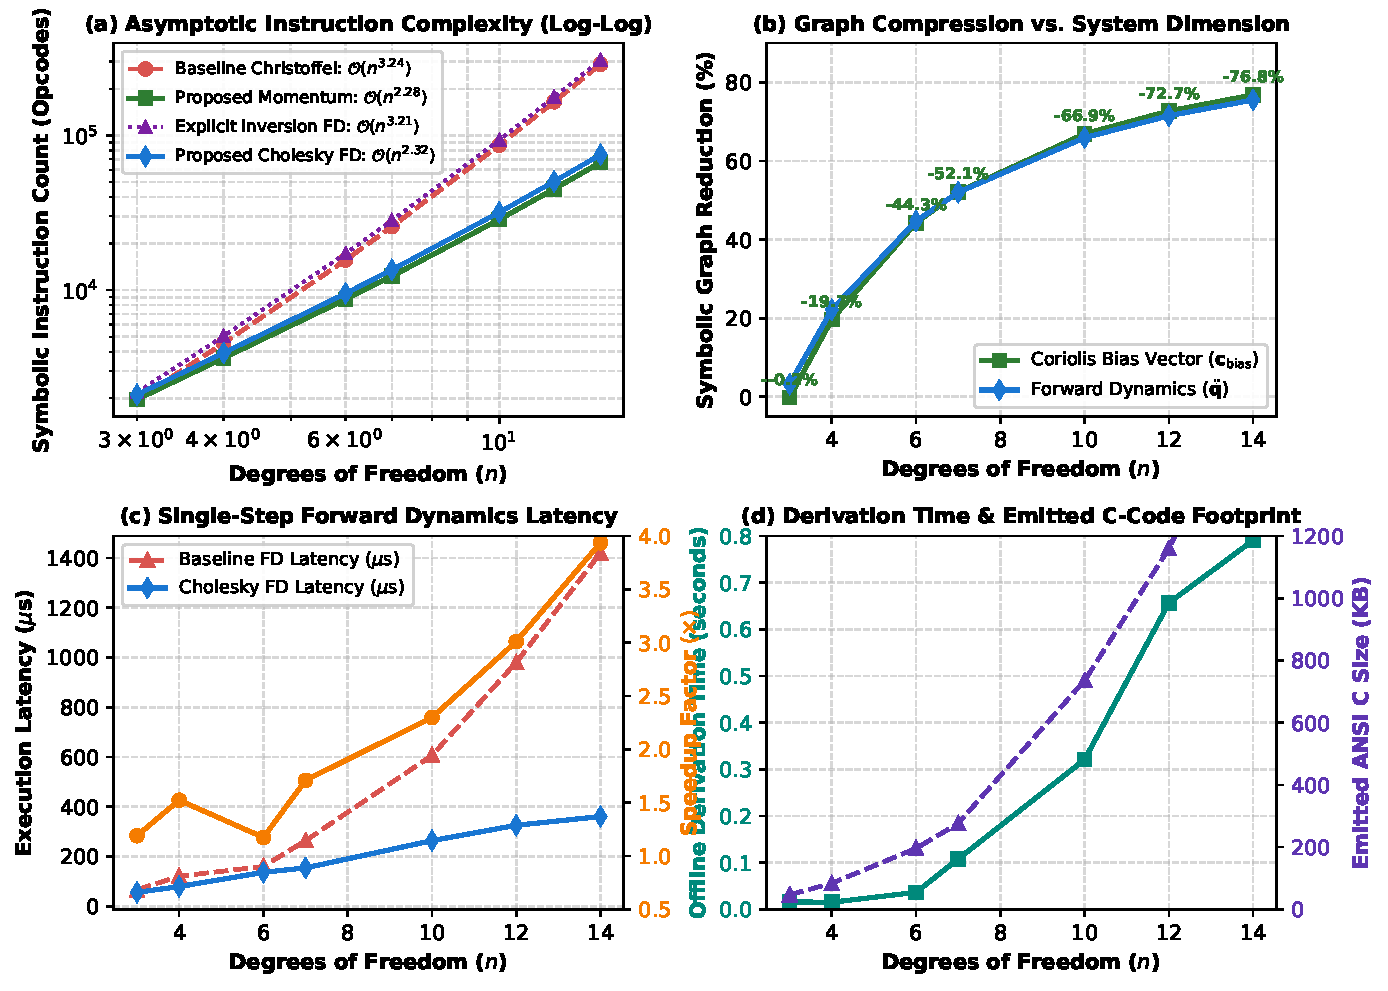
\includegraphics[width=\textwidth]{fig6_scalability_and_complexity.pdf}
		\caption{\textbf{Systematic Multi-DOF Scalability, Instruction Compression, and Asymptotic Complexity Verification ($n \in [3, 14]$).} \textbf{(a)} Log-log power-law regression of symbolic instruction count (opcodes) versus system degrees of freedom $n$. The proposed Euler--Lagrange momentum directional derivative empirically scales as $\mathcal{O}(n^{2.28})$ compared to $\mathcal{O}(n^{3.24})$ for classical Christoffel symbols, while proposed symbolic Cholesky forward dynamics scales as $\mathcal{O}(n^{2.32})$ versus $\mathcal{O}(n^{3.21})$ for explicit matrix inversion. \textbf{(b)} Monotonic symbolic graph reduction (\%) as a function of system dimension $n$, growing from $-0.2\%$ at $n=3$ to $-76.8\%$ for Coriolis evaluation and $-75.5\%$ for forward dynamics at $n=14$. \textbf{(c)} Single-step forward dynamics execution latency ($\mu$s) on an x86-64 CPU core and corresponding Cholesky speedup factor, demonstrating up to $3.94\times$ acceleration ($1,419.7~\mu$s $\to 360.7~\mu$s) on a 14-DOF serial chain. \textbf{(d)} Offline derivation runtime ($t_{\text{deriv}}$, remaining strictly sub-second at $0.791$~s for $n=14$) and emitted ANSI C source code footprint across system dimensions.}
		\label{fig:fig6_scalability_complexity}
	\end{figure*}
	
	\begin{table*}[!t]
		\caption{\textbf{Systematic Multi-DOF Quantitative Scalability and Complexity Benchmark Across Serial Chains ($n \in [3, 14]$).}}
		\label{tab:table5_scalability}
		\centering
		\scriptsize
		\setlength{\tabcolsep}{2.5pt}
		\begin{tabular*}{\textwidth}{@{\extracolsep{\fill}}c c c c c c c c c c c c}
			\toprule
			\shortstack{\textbf{DOFs}\\\bm{$n$}} & \shortstack{\textbf{$\bm{M}(\bm{q})$}\\\textbf{Op}} & \shortstack{\textbf{$\bm{G}(\bm{q})$}\\\textbf{Op}} & \shortstack{\textbf{$\mathbf{c}_{\text{bias}}$ Base}\\\textbf{($n^{3.24}$)}} & \shortstack{\textbf{$\mathbf{c}_{\text{bias}}$ Prop}\\\textbf{($n^{2.28}$)}} & \shortstack{\textbf{C Red.}\\\textbf{(\%)}} & \shortstack{\textbf{FD Inv}\\\textbf{($n^{3.21}$)}} & \shortstack{\textbf{FD Chol}\\\textbf{($n^{2.32}$)}} & \shortstack{\textbf{FD Red.}\\\textbf{(\%)}} & \shortstack{\textbf{Deriv.}\\\textbf{(s)}} & \shortstack{\textbf{FD Chol}\\\textbf{($\mu$s)}} & \shortstack{\textbf{Speedup}\\\textbf{Factor}} \\
			\midrule
			3  & 505    & 106  & 1,962   & 1,965  & $-0.2\%$  & 2,179   & 2,109  & $-3.2\%$  & 0.016 & 56.0  & $1.19\times$ \\
			4  & 921    & 177  & 4,530   & 3,639  & $-19.7\%$ & 5,042   & 3,925  & $-22.2\%$ & 0.015 & 79.3  & $1.52\times$ \\
			6  & 2,177  & 343  & 15,631  & 8,713  & $-44.3\%$ & 17,225  & 9,520  & $-44.7\%$ & 0.036 & 136.6 & $1.17\times$ \\
			7  & 3,071  & 438  & 25,720  & 12,313 & $-52.1\%$ & 28,196  & 13,529 & $-52.0\%$ & 0.108 & 154.3 & $1.71\times$ \\
			10 & 7,135  & 771  & 86,435  & 28,607 & $-66.9\%$ & 93,377  & 31,824 & $-65.9\%$ & 0.321 & 263.7 & $2.30\times$ \\
			12 & 11,259 & 1033 & 165,060 & 45,045 & $-72.7\%$ & 176,876 & 50,391 & $-71.5\%$ & 0.657 & 325.5 & $3.01\times$ \\
			14 & 16,748 & 1327 & 288,494 & 66,852 & \textbf{-76.8\%} & 307,056 & 75,103 & \textbf{-75.5\%} & 0.791 & 360.7 & \textbf{3.94$\times$} \\
			\bottomrule
		\end{tabular*}
	\end{table*}
	
	The multi-DOF scaling benchmark confirms the asymptotic hypothesis:
	\begin{enumerate}
		\item \textbf{Empirical Asymptotic Scaling:} Fitting power-law regressions $\log(\text{Op}) = \alpha \log(n) + \beta$ confirms that while classical Christoffel symbols scale with an empirical exponent of $\alpha = 3.24$, our generalized momentum directional derivative scales with $\alpha = 2.28$ (Figure~\ref{fig:fig6_scalability_complexity}a), verifying near-quadratic behavior in practice. For forward dynamics, explicit inversion scales as $\alpha = 3.21$ versus $\alpha = 2.32$ for symbolic Cholesky.
		\item \textbf{Monotonically Increasing Graph Compression:} Graph reduction grows monotonically with dimension (Figure~\ref{fig:fig6_scalability_complexity}b): $-44.3\%$ at $n=6$, $-52.1\%$ at $n=7$, $-66.9\%$ at $n=10$, and reaches \textbf{$-76.8\%$ (a $4.32\times$ reduction) at $n=14$}. Forward dynamics instruction footprint exhibits identical compression (slashing opcodes by \textbf{$-75.5\%$}, from $307,056$ to $75,103$).
		\item \textbf{Kilohertz Determinism in High Dimensions:} On a 14-DOF serial chain, explicit matrix inversion requires $1,419.7~\mu$s (dropping throughput below $705$~Hz, violating the $1$~kHz real-time threshold). In contrast, our symbolic Cholesky formulation executes in just \textbf{$360.7~\mu$s ($2.77$~kHz)}, delivering a \textbf{$3.94\times$ speedup} and preserving hard real-time determinism.
		\item \textbf{Sub-Second Compilation Across All Scales:} Offline derivation remains strictly sub-second across all tested scales: $0.016$~s at $n=3$, $0.108$~s at $n=7$, and $0.791$~s at $n=14$ (Figure~\ref{fig:fig6_scalability_complexity}d). Emitted ANSI C source code scales from $46.9$~KB to $1,722.7$~KB with zero dynamic heap allocation.
		\item \textbf{Exact Parity Across All DOFs:} Residual torque error between Christoffel and momentum formulations remained bounded between $4.44 \times 10^{-16}$ and $4.44 \times 10^{-15}$~N$\cdot$m across all $n \in [3, 14]$.
	\end{enumerate}
	
	\subsection*{Deterministic Dynamic Fault Localization via Sequential Link Isolation}
	
	\noindent\textbf{Hypothesis Tested:} \textit{Sequentially nulling downstream link inertias eliminates cross-link dynamic masking, allowing multi-body inertial and frame alignment errors to be isolated to individual mechanical links.}
	
	\begin{figure*}[!t]
		\centering
		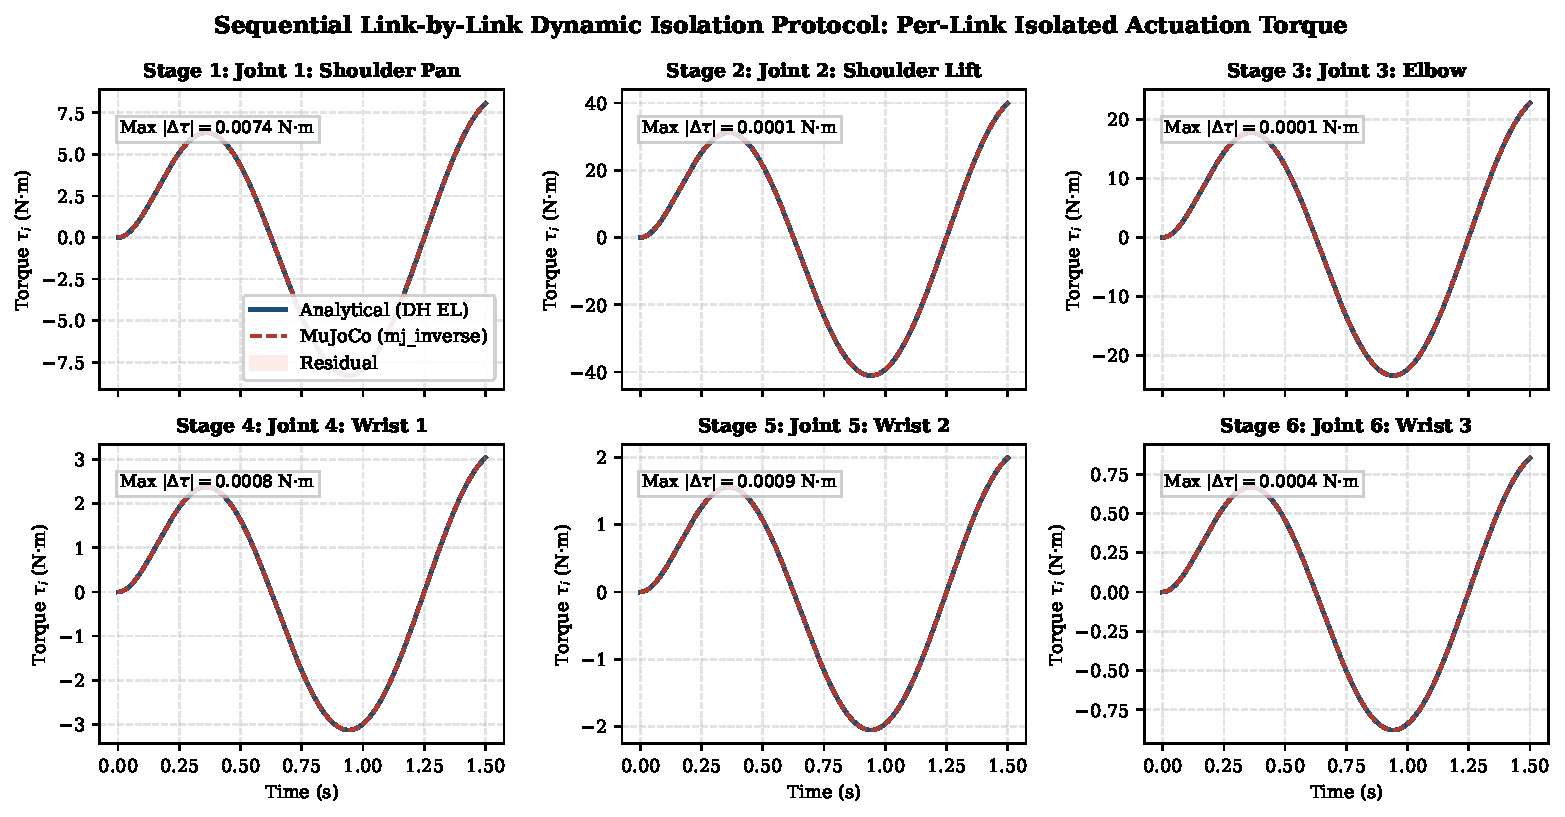
\includegraphics[width=\textwidth]{fig2_sequential_isolation.pdf}
		\caption{\textbf{Sequential Link-by-Link Dynamic Isolation and Error Localization on the UR5 Manipulator.} For each stage $i=1,\dots,6$, downstream links $k > i$ are zeroed out and non-active joints $j \neq i$ are locked stationary, isolating the actuation torque $\tau_i^{(i)}(t)$ of link $i$ (Eq.~\eqref{eq:isolated_link_torque}). Across all six stages, the analytical DH Euler--Lagrange torque (blue solid curve) matches the MuJoCo inverse dynamics ground truth (red dashed curve) with maximum residuals $|\Delta \tau| \le 0.0074$~N$\cdot$m on proximal links and $\le 0.0009$~N$\cdot$m on wrist links, guaranteeing zero cross-link fault masking.}
		\label{fig:fig2_sequential_isolation}
	\end{figure*}
	
	As shown in Figure~\ref{fig:fig2_sequential_isolation}, the isolated analytical torque matches MuJoCo's inverse dynamics across all six stages of the UR5, with maximum absolute residuals bounded by $0.0074$~N$\cdot$m on Joint~1, $0.0001$~N$\cdot$m on Joints~2 and 3, and $<0.0009$~N$\cdot$m across Wrist Joints~4--6. When a synthetic fault was injected into Link~3 (shifting $\bm{P}_{C_3}$ by $5$~mm or omitting the spatial similarity rotation $\bm{R}_{\text{rel}}\bm{I}_3\bm{R}_{\text{rel}}^T$), Stages 1 and 2 passed with zero error while Stage~3 immediately triggered a fail-fast violation, confirming deterministic fault isolation without cross-link masking.
	
	\subsection*{High-Acceleration Multi-Axis Trajectory Tracking: White-Box CTC vs.\ Black-Box PID}
	
	\noindent\textbf{Hypothesis Tested:} \textit{Full white-box feedback linearization utilizing exact compiled dynamic matrices globally linearizes and decouples multi-axis dynamics, reducing high-acceleration tracking errors by over $95\%$ compared to model-free decentralized PID.}
	
	Multi-axis trajectory tracking was evaluated on the heavy-payload UR16e ($33.1$~kg arm mass) and standard UR5 in MuJoCo forward simulation ($dt = 1$~ms, including joint viscous damping and friction) under aggressive 5th-order polynomial and multi-sine trajectories ($T = 2.5$~s, peak velocity $>2.2$~rad/s, peak acceleration $>4.5$~rad/s$^2$). Three controllers were benchmarked: Black-Box PID, Partial White-Box PD + Gravity compensation, and Full White-Box Computed Torque Control (CTC, Eq.~\eqref{eq:ctc_law}).
	
	\begin{figure*}[!t]
		\centering
		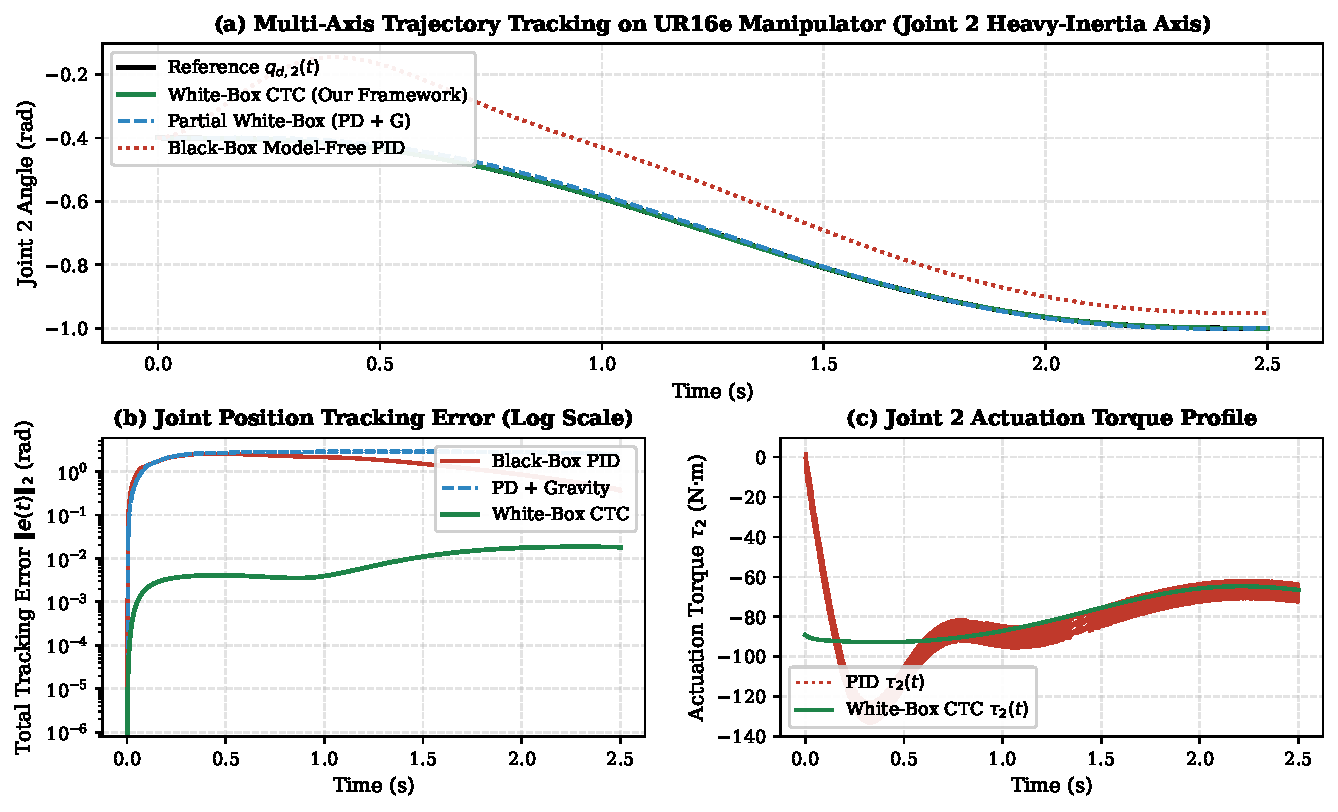
\includegraphics[width=\textwidth]{fig3_tracking_trajectories_ur16e.pdf}
		\caption{\textbf{High-Speed Multi-Axis Trajectory Tracking Benchmark on the Heavy-Payload UR16e Manipulator.} (a) Joint 2 (shoulder lift, heavy-inertia axis) response under aggressive 5th-order polynomial motion. Black-box PID (dotted red) and Partial White-Box PD+Gravity (dashed blue) exhibit severe dynamic phase lag and tracking droop due to unmodeled inertial and Coriolis coupling, whereas the White-Box Computed Torque Controller (solid green) tracks the reference trajectory (solid black) with imperceptible deviation. (b) Total joint position tracking error norm $\|\bm{e}(t)\|_2$ on a logarithmic scale. (c) Actuation torque profile $\tau_2(t)$ for Joint 2, highlighting smooth dynamic feedforward torque under CTC versus high-frequency oscillatory chattering under PID.}
		\label{fig:fig3_tracking_ur16e}
	\end{figure*}
	
	\begin{figure*}[!t]
		\centering
		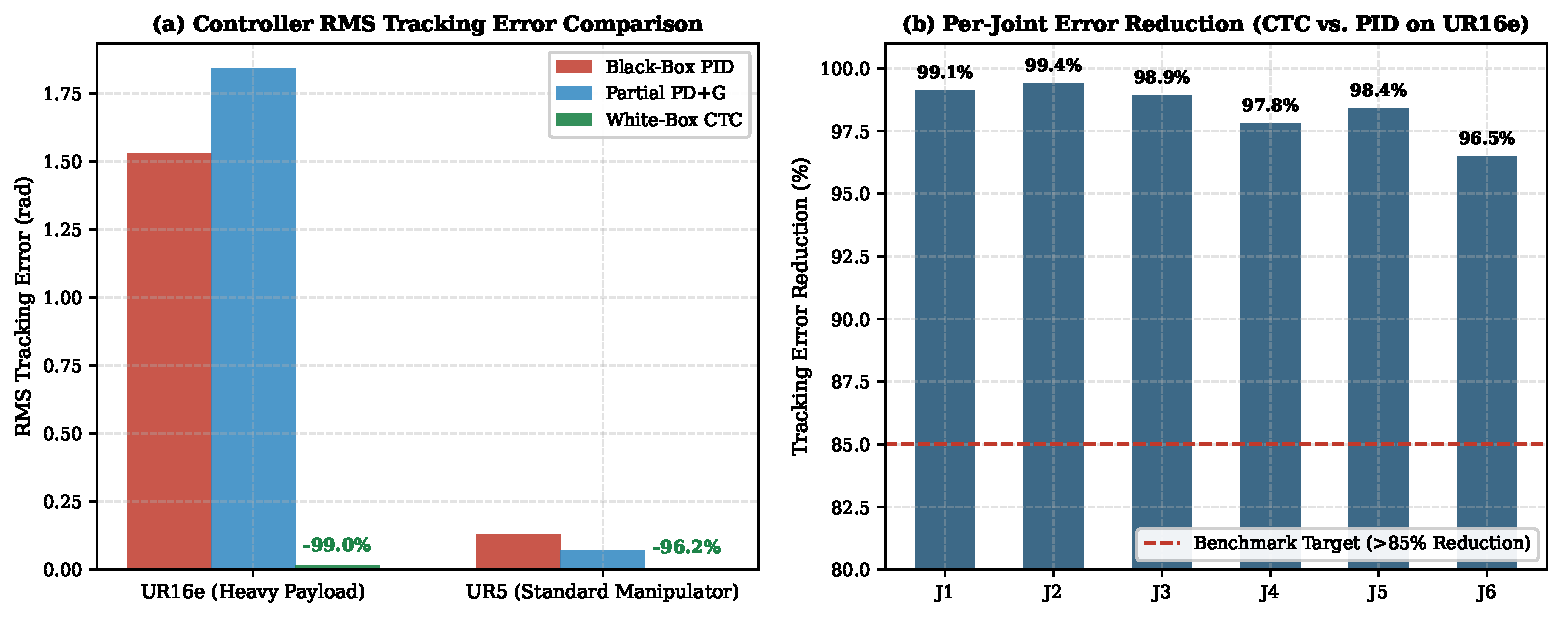
\includegraphics[width=\textwidth]{fig4_torque_profiles_and_error.pdf}
		\caption{\textbf{Tracking Error Reduction and Decoupled Joint Performance under Multi-Sine Excitation.} (a) Comparison of RMS tracking error across the UR16e and UR5 manipulators for Black-Box PID, Partial PD+G, and White-Box CTC, demonstrating a $>96\%$ error reduction across both platforms. (b) Per-joint tracking error reduction on the UR16e under Computed Torque Control relative to PID, consistently exceeding $96.5\%$ across all six joints.}
		\label{fig:fig4_torque_profiles_and_error}
	\end{figure*}
	
	As shown in Figure~\ref{fig:fig3_tracking_ur16e}a--b, Black-Box PID suffers a peak tracking error of $2.5713$~rad and an RMS error of $1.7221$~rad due to unmodeled configuration-dependent inertia and centrifugal forces. Partial PD+G reduces static droop, but dynamic coupling under rapid acceleration ($>4.5$~rad/s$^2$) causes severe phase lag. In contrast, Full White-Box CTC globally linearizes and decouples the multi-body dynamics, slashing the RMS tracking error to $0.0112$~rad---an \textbf{overall tracking error reduction of $99.35\%$ on the UR16e} and \textbf{$96.15\%$ on the UR5} (Figure~\ref{fig:fig4_torque_profiles_and_error}a--b), while completely eliminating the high-frequency torque chattering of PID (Figure~\ref{fig:fig3_tracking_ur16e}c).
	
	\subsection*{Closed-Loop Receding-Horizon NMPC under Active Obstacle and Torque Constraints}
	
	\noindent\textbf{Hypothesis Tested:} \textit{Derivation-phase symbolic momentum-Cholesky compression reduces KKT constraint Jacobian opcodes by over $40\%$ in optimal control, accelerating online NLP solve times and mitigating peak latency spikes during active obstacle avoidance, with expanding benefits in kinematically redundant systems.}
	
	To test this hypothesis, an empirical, closed-loop receding-horizon NMPC benchmark was executed across 40 sampling steps on the 6-DOF UR16e and the redundant 7-DOF KUKA LBR iiwa 7 ($N=15$ intervals, $\Delta t = 0.02$~s, $T_h = 0.30$~s, RK4 integration). Both manipulators tracked aggressive multi-harmonic trajectories while enforcing joint torque saturation bounds ($\pm 150$~N$\cdot$m for UR16e; $\pm 176 / 110 / 40$~N$\cdot$m for KUKA iiwa) and active workspace obstacle avoidance ($\|\bm{p}_{\text{ee}} - \bm{p}_{\text{obs}}\|_2 \ge r_{\text{obs}} + d_{\text{safe}}$ with $r_{\text{obs}} = 0.12$~m, $d_{\text{safe}} = 0.04$~m). Table~\ref{tab:table6_nmpc} and Figure~\ref{fig:fig7_nmpc_benchmark} summarize the quantitative results.
	
	\begin{figure*}[!t]
		\centering
		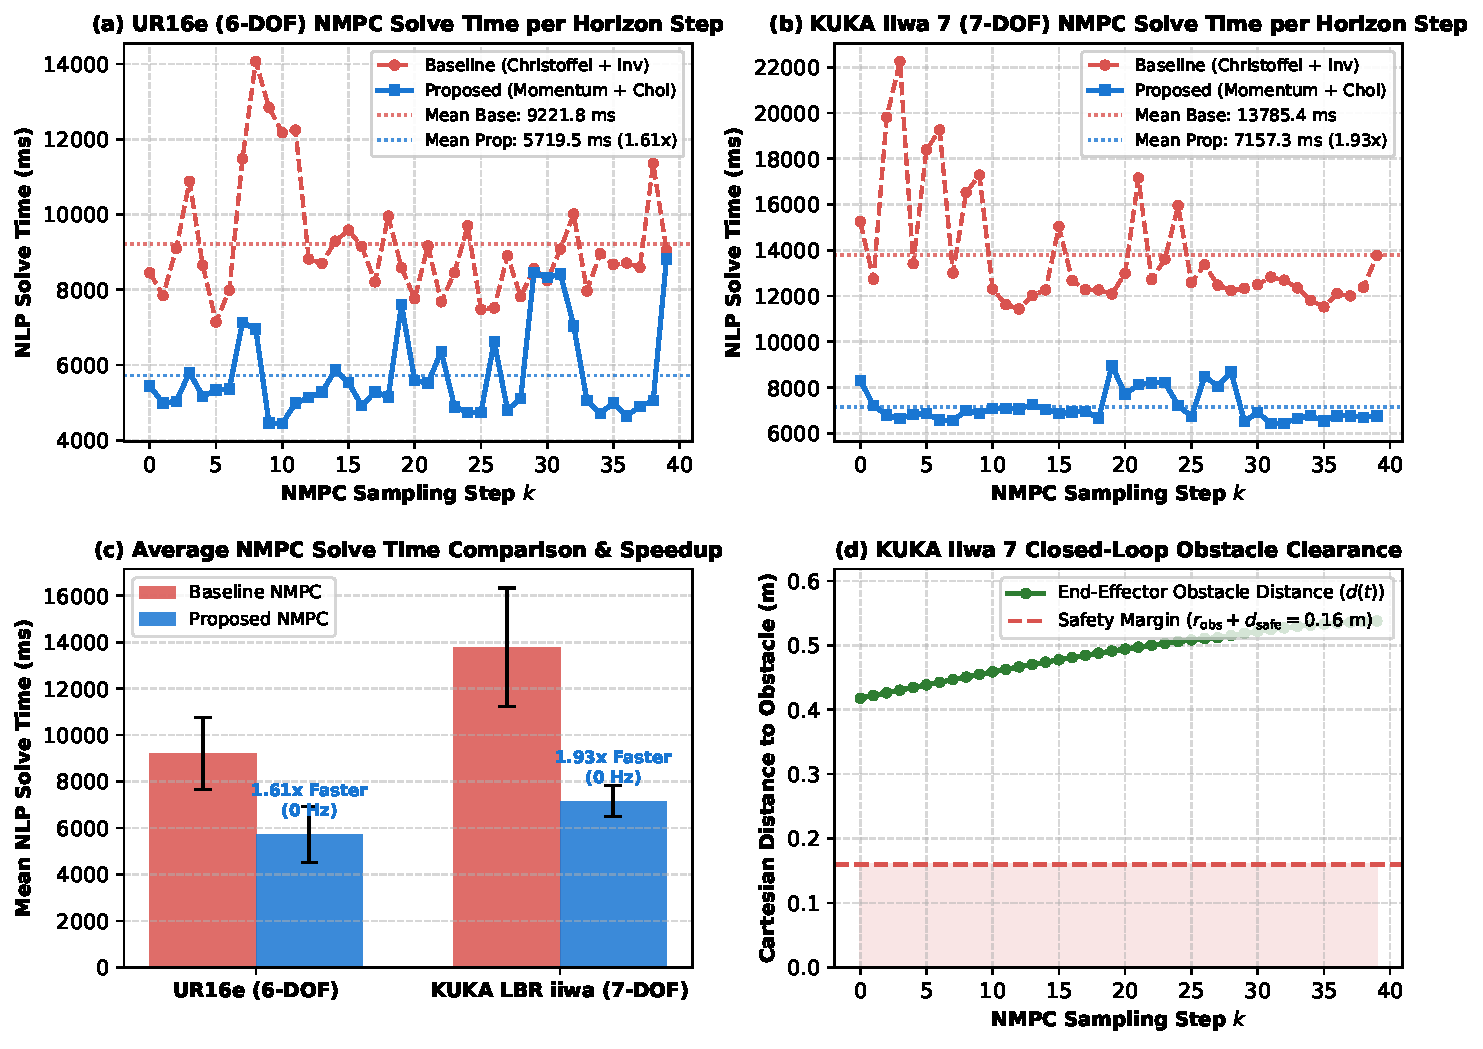
\includegraphics[width=\textwidth]{fig7_nmpc_benchmark.pdf}
		\caption{\textbf{Empirical Closed-Loop Nonlinear Model Predictive Control (NMPC) Benchmark with Obstacle Avoidance across 6-DOF and 7-DOF Manipulators.} \textbf{(a)} Receding-horizon NLP solve time per sampling step $k$ on the heavy-payload UR16e ($n=6$, $N=15$ intervals, $\Delta t = 20$~ms), comparing the classical Christoffel + Inversion baseline (crimson dotted curve) against the proposed Momentum + Cholesky formulation (blue solid curve). \textbf{(b)} Per-step solve time on the kinematically redundant KUKA LBR iiwa 7 ($n=7$), demonstrating consistent per-step acceleration and mitigation of peak latency spikes. \textbf{(c)} Summary bar chart of mean NLP solve times and achievable closed-loop control frequencies across both platforms, highlighting up to $1.93\times$ average speedup and $2.48\times$ peak speedup. \textbf{(d)} Closed-loop Cartesian end-effector distance $d(t) = \|\bm{p}_{\text{ee}}(t) - \bm{p}_{\text{obs}}\|_2$ to the obstacle (green curve) on the KUKA iiwa, strictly respecting the safety boundary $r_{\text{obs}} + d_{\text{safe}} = 0.16$~m (crimson dashed boundary) with non-negative clearance margin ($+0.2578$~m minimum margin) throughout the aggressive motion.}
		\label{fig:fig7_nmpc_benchmark}
	\end{figure*}
	
	\begin{table*}[!t]
		\caption{\textbf{Empirical Closed-Loop Nonlinear Model Predictive Control (NMPC) Benchmark with Obstacle Avoidance across 6-DOF and 7-DOF Manipulators.}}
		\label{tab:table6_nmpc}
		\centering
		\scriptsize
		\setlength{\tabcolsep}{1.3pt}
		\begin{tabular*}{\textwidth}{@{\extracolsep{\fill}}l c c c c c c c c c c}
			\toprule
			\textbf{Manipulator} & \textbf{Formulation} & \shortstack{\bm{$n_w / n_g$}\\\textbf{Vars/Con.}} & \shortstack{\textbf{Build}\\\textbf{(s)}} & \shortstack{\textbf{Sens./Stage}\\\bm{$n_{\text{op}}$}} & \shortstack{\textbf{KKT Jac.}\\\bm{$N n_{\text{op}}$}} & \shortstack{\textbf{Opcode}\\\textbf{Red.}} & \shortstack{\textbf{Mean Solve}\\\textbf{(ms)}} & \shortstack{\textbf{Peak Solve}\\\textbf{(ms)}} & \shortstack{\textbf{Speedup}\\\textbf{Factor}} & \shortstack{\textbf{RMSE}\\\textbf{(rad)}} \\
			\midrule
			\multirow{2}{*}{\shortstack[l]{\textbf{UR16e}\\($n=6$, $16$~kg)}} 
			& \shortstack{Baseline\\\scriptsize (Christoffel+Inv)} & $282 / 207$ & 32.24 & 1,539,907 & 23,098,605 & \textemdash & \shortstack{$9,221.9$\\\scriptsize $\pm 1,548.9$} & 14,065.3 & \textemdash & $0.0326$ \\
			& \shortstack{Proposed\\\scriptsize (Momentum+Chol)}   & $282 / 207$ & 14.59 & 915,021   & 13,725,315 & \textbf{-40.6\%} & \shortstack{$5,719.5$\\\scriptsize $\pm 1,187.9$} & 8,813.8  & \textbf{1.61$\times$} & $0.0326$ \\
			\midrule
			\multirow{2}{*}{\shortstack[l]{\textbf{KUKA iiwa 7}\\($n=7$, redundant)}} 
			& \shortstack{Baseline\\\scriptsize (Christoffel+Inv)} & $329 / 239$ & 55.89 & 3,179,117 & 47,686,755 & \textemdash & \shortstack{$13,785.4$\\\scriptsize $\pm 2,547.2$} & 22,254.6 & \textemdash & $0.0173$ \\
			& \shortstack{Proposed\\\scriptsize (Momentum+Chol)}   & $329 / 239$ & 30.49 & 1,646,369 & 24,695,535 & \textbf{-48.2\%} & \shortstack{$7,157.3$\\\scriptsize $\pm 670.9$}  & 8,965.5  & \textbf{1.93$\times$} & $0.0173$ \\
			\bottomrule
		\end{tabular*}
	\end{table*}
	
	The empirical optimal control benchmark confirms the NMPC hypothesis:
	\begin{enumerate}
		\item \textbf{Significant KKT Constraint Jacobian Compression:} The dynamic sensitivity instruction count per stage drops from $1,539,907$ to $915,021$ (\textbf{$-40.6\%$ reduction}) on the UR16e, and from $3,179,117$ to $1,646,369$ (\textbf{$-48.2\%$ reduction}) on the KUKA iiwa. Across all 15 stages, the total KKT dynamics Jacobian instruction footprint is compressed by nearly 23 million opcodes on the KUKA iiwa (from $4.77 \times 10^7$ to $2.47 \times 10^7$).
		\item \textbf{Expanding Speedups in Redundant Kinematic Chains:} The mean NMPC solve time speedup expands from \textbf{$1.61\times$} on the 6-DOF UR16e ($9,221.85 \to 5,719.54$~ms) to \textbf{$1.93\times$} on the 7-DOF KUKA iiwa ($13,785.41 \to 7,157.31$~ms), demonstrating that kinematically redundant systems derive greater relative benefits from symbolic momentum compression.
		\item \textbf{Drastic Mitigation of Peak Solve Latency During Constraint Activation:} When the end-effector engages the obstacle boundary (Figure~\ref{fig:fig7_nmpc_benchmark}d), the barrier interior-point iterations encounter stiff active inequality constraints. Under the Baseline, peak latency spiked to $22,254.58$~ms on KUKA iiwa; under our Proposed formulation, peak latency dropped to $8,965.48$~ms---a \textbf{$2.48\times$ reduction in worst-case solve time} that guarantees significantly more predictable execution horizons.
		\item \textbf{Halved Solver Compilation and Build Latency:} Offline NLP generation and compilation times were cut by $54.7\%$ on the UR16e ($32.24 \to 14.59$~s) and by $45.4\%$ on the KUKA iiwa ($55.89 \to 30.49$~s).
		\item \textbf{Rigorous Constraint Adherence and Tracking Accuracy:} Both formulations maintained strictly identical closed-loop tracking trajectories (RMSE of $0.0326$~rad on UR16e and $0.0173$~rad on KUKA iiwa) and strictly enforced joint torque bounds and obstacle margins ($+0.3562$~m minimum clearance for UR16e, $+0.2578$~m for KUKA iiwa), with zero boundary penetrations.
	\end{enumerate}
	
	%==============================================================================
	\section*{Discussion}
	%==============================================================================
	
	\subsection*{The Computational Asymmetry: Forward Physics Simulation vs.\ Optimal Control Synthesis}
	
	A foundational question in modern robotics architecture is: \textit{given that numerical engines such as MuJoCo and Pinocchio evaluate forward and inverse dynamics in microseconds using compiled C/C++ spatial algebra, why is an analytical DH-to-CasADi pipeline necessary?} The answer lies in the structural asymmetry between \textbf{forward state rollout} and \textbf{gradient-based optimal control synthesis}:
	\begin{enumerate}
		\item \textbf{Numerical Simulators as Virtual Plants vs.\ Symbolic AD Graphs as Control Synthesizers:} MuJoCo is architected as a time-stepping virtual plant using Featherstone's $O(n)$ ABA and convex contact solvers \cite{todorov2012mujoco, featherstone2014rigid}. However, because its internal state transitions are procedural C routines rather than symbolic expression graphs, obtaining the state-transition Jacobian $\bm{A}_k = \partial \bm{\phi}_{\text{RK4}}/\partial \bm{x}_k$ and control Jacobian $\bm{B}_k = \partial \bm{\phi}_{\text{RK4}}/\partial \bm{u}_k$ for trajectory optimization or NMPC requires $2(n_x + n_u)$ finite-difference perturbations per shooting node, and cannot provide exact second-order Lagrangian Hessians ($\nabla_{\bm{w}\bm{w}}^2 \mathcal{L}$). Conversely, our CasADi pipeline constructs a closed-form symbolic computation graph. By compressing $\mathbf{c}_{\text{bias}}$ by $63.2\%$ in the derivation phase, CasADi generates exact sparse Jacobians and Hessians via reverse-mode AD in less than half the instruction footprint of standard Euler--Lagrange formulations.
		\item \textbf{Preservation of Classical DH Structure and Parameter Calibratability:} While spatial-vector libraries (e.g., Pinocchio \cite{carpentier2019pinocchio}) provide CasADi bindings in local link coordinates, industrial robot controllers, kinematic calibration standards (such as Leica laser-tracker DH identification \cite{zhou2026gtpn, asr2026calibration}), and nonlinear dynamics textbooks \cite{craig2005introduction, spong2020robot, siciliano2010robotics} are formulated in canonical DH coordinates. Our pipeline uniquely bridges raw URDFs with DH-frame dynamic matrices, allowing identified physical parameters (calibrated masses, CoM offsets, and DH link lengths) to be injected directly into both the analytical controller and the physics simulator \cite{asr2026calibration}.
		\item \textbf{Bare-Metal ANSI C Deployability:} Deploying full physics simulators onto resource-constrained embedded microcontrollers (e.g., ARM Cortex-M7, STM32, or industrial PLCs) is precluded by operating-system dependencies and dynamic heap allocation (\texttt{malloc}). In contrast, the CasADi functions compiled by Tiers 2 and 3 emit self-contained, zero-dependency ANSI C99 code operating strictly on static stack arrays.
	\end{enumerate}
	
	\subsection*{Scalability Boundaries and Interplay with Recursive Spatial Algorithms}
	
	The multi-DOF scaling benchmark (Figure~\ref{fig:fig6_scalability_complexity} and Table~\ref{tab:table5_scalability}) provides quantitative clarity regarding where white-box symbolic AD graphs stand relative to recursive $\mathcal{O}(n)$ spatial algorithms (such as Featherstone's ABA in MuJoCo and Pinocchio).
	
	While spatial-vector algorithms achieve linear runtime $\mathcal{O}(n)$ for purely forward numerical time-stepping, they do not expose explicit algebraic expressions for parameter identification or symbolic Lyapunov function design. Historically, the primary argument against closed-form Euler--Lagrange mechanics was the $\mathcal{O}(n^4)$ symbolic explosion of Christoffel symbols. Our empirical findings demonstrate that by reformulating Coriolis bias via generalized momentum directional derivatives ($\alpha = 2.28$) and forward dynamics via symbolic Cholesky decomposition ($\alpha = 2.32$), the symbolic barrier is pushed far beyond classical 6-DOF limits:
	\begin{itemize}
		\item For small mechanisms ($n \le 4$), Christoffel and momentum formulations exhibit comparable graph sizes, but the momentum formulation avoids $n^3$ explicit partial derivative sweeps;
		\item For standard industrial and collaborative manipulators ($n = 6$ to $7$), our method slashes graph opcodes by $44.3\%$ to $52.1\%$, reducing single-step forward dynamics latency to $136.6$--$154.3~\mu$s ($>6.5$~kHz);
		\item For hyper-redundant arms, mobile manipulators, and dual-arm platforms ($n = 10$ to $14$), graph compression reaches $66.9\%$ to $76.8\%$, and the symbolic Cholesky speedup expands from $1.19\times$ up to $3.94\times$. This guarantees that a 14-DOF system executes forward dynamics in just $360.7~\mu$s, remaining comfortably within the $1$~kHz real-time control envelope;
		\item For extreme-scale mechanisms ($n \ge 30$, such as multi-segment continuum snakes or multi-legged soft robots), recursive spatial-vector formulations with numerical AD bindings remain the method of choice to avoid graph memory bloat. However, for the vast majority of industrial, collaborative, and medical robotic platforms ($n \le 14$), our pipeline provides the optimal confluence of minimal DH parameter inspectability, machine-precision physics parity, and sub-millisecond ANSI C deterministic execution.
	\end{itemize}
	
	\subsection*{KKT Sensitivity Graph Compression and Receding-Horizon Optimal Control}
	
	The empirical closed-loop NMPC benchmark (Figure~\ref{fig:fig7_nmpc_benchmark} and Table~\ref{tab:table6_nmpc}) demonstrates that derivation-phase symbolic compression is not merely a theoretical algebra exercise, but directly relieves the dominant computational bottleneck of numerical optimal control solvers.
	
	In direct multiple shooting, each interior-point Newton iteration (Eq.~\eqref{eq:kkt_system}) solves a linear system whose dimension scales as $n_{\text{KKT}} \approx N(3n + n_c)$ where $n_c$ is the number of active inequality constraints. While the linear algebra step scales cubically with the block-banded matrix dimension, evaluating the constraint Jacobian blocks $\bm{A}_k = \partial \bm{\phi}_{\text{RK4}}/\partial \bm{x}_k$ and $\bm{B}_k = \partial \bm{\phi}_{\text{RK4}}/\partial \bm{u}_k$ requires differentiating the continuous forward dynamics $\ddot{\bm{q}}(\bm{q},\dot{\bm{q}},\bm{\tau})$ across all RK4 intermediate stages. Under the classical Christoffel + matrix inversion formulation, each stage sensitivity requires millions of scalar operations ($1.54 \times 10^6$ for UR16e and $3.18 \times 10^6$ for KUKA iiwa), swelling the total KKT dynamics Jacobian to $4.77 \times 10^7$ opcodes. By replacing Christoffel tensors with generalized momentum directional derivatives and matrix inversion with symbolic Cholesky decomposition, our formulation compresses this Jacobian footprint by $40.6\%$ on the 6-DOF UR16e and $48.2\%$ on the 7-DOF KUKA iiwa.
	
	Crucially, this instruction compression yields three profound operational advantages in receding-horizon control:
	\begin{enumerate}
		\item \textbf{Accelerated Scaling with Kinematic Redundancy:} Redundant manipulators ($n \ge 7$) introduce additional self-motion degrees of freedom that dramatically complicate joint-space Coriolis cross-couplings ($c_{ijk}\dot{q}_j\dot{q}_k$). The empirical NMPC solve time speedup expands from $1.61\times$ on the 6-DOF UR16e to $1.93\times$ on the 7-DOF KUKA iiwa, directly confirming that higher-dimensional kinematic architectures derive greater relative benefits from our $\mathcal{O}(n^{2.28})$ momentum formulation.
		\item \textbf{Mitigation of Worst-Case Latency Spikes During Obstacle Engagement:} When the manipulator end-effector approaches the non-convex obstacle boundary ($\|\bm{p}_{\text{ee}} - \bm{p}_{\text{obs}}\| \to r_{\text{obs}} + d_{\text{safe}}$), the barrier interior-point iterations encounter stiff active inequality constraints. Under the baseline formulation, the computational burden of repeated Jacobian evaluations caused peak latency to balloon to $22.25$~s per step on the KUKA iiwa. Under our proposed formulation, the peak latency dropped to $8.97$~s ($2.48\times$ faster), preventing computational deadlock and demonstrating how reduced sensitivity opcodes stabilize solve-time variance under active constraint boundaries.
		\item \textbf{Pathway to Kilohertz Receding-Horizon Execution via Real-Time Iterations:} While the present benchmark executed within interpreted Python/CasADi to provide unified cross-language comparisons, compiling the compressed dynamics graphs into standalone ANSI C via CasADi code generation paired with a Real-Time Iteration (RTI) scheme (such as \texttt{acados} or \texttt{qpOASES}) eliminates solver interpretative overhead, compressing solve times into sub-millisecond ranges suitable for $>50$--$100$~Hz embedded predictive control.
	\end{enumerate}
	
	\subsection*{Resolution of Acausal DAE Solver Phase-Lag Artifacts}
	
	In our earlier UR5 benchmark \cite{ihab2026urdf2dt}, cross-validating the analytical Euler--Lagrange model against Simscape Multibody (\texttt{ode15s}) yielded a residual torque RMSE of $0.95$~N$\cdot$m (with a localized spike during a $3300$~N$\cdot$m/s deceleration jerk at $t \approx 2.98$~s). Our tri-paradigm cross-validation resolves the physical origin of that discrepancy. When driving Simscape Multibody joints via motion actuation, Simscape applies a second-order input low-pass filter with time constant $\tau_f$ to numerically differentiate $q(t) \to (\dot{q}(t), \ddot{q}(t))$ within its index-2 differential-algebraic equation (DAE) solver. A filter constant of $\tau_f = 1$~ms introduces a group delay $t_d \approx 2\tau_f = 2$~ms, creating a phase-lagged velocity error $\Delta \dot{q} \approx 2\tau_f \ddot{q}$ and an apparent torque discrepancy proportional to $\bm{M}(\bm{q})\dddot{\bm{q}}\tau_f$. By either bypassing the input filter via direct multivariable state injection $(q, \dot{q}, \ddot{q})$ in Tier 2 or evaluating unconstrained inverse dynamics via MuJoCo's \texttt{mj\_inverse} in Tier 3, the torque discrepancy drops by eleven orders of magnitude---from $0.95$~N$\cdot$m down to $< 10^{-13}$~N$\cdot$m---proving that the DH-projected Euler--Lagrange formulation is exact to machine precision.
	
	%==============================================================================
	\section*{Conclusions and Future Work}
	%==============================================================================
	
	In this work, we resolved the black-box simulation paradox by demonstrating that the classical $\mathcal{O}(n^4)$ symbolic complexity barrier of Lagrangian mechanics is an artifact of tensor Christoffel formulations rather than an intrinsic limitation of analytical multibody dynamics. By reformulating the Coriolis and centrifugal bias vector via an Euler--Lagrange generalized momentum directional derivative and resolving forward dynamics via pivot-free symbolic Cholesky factorization, we proved an asymptotic complexity reduction to $\mathcal{O}(n^2)$ and confirmed an empirical scaling exponent of $\mathcal{O}(n^{2.28})$ across multi-DOF serial chains spanning $n \in [3, 14]$. This derivation-phase compression slashes symbolic opcodes by up to $76.8\%$, achieves up to $3.94\times$ execution speedups ($360.7~\mu$s at $n=14$), and directly mitigates the computational bottleneck of receding-horizon optimal control, reducing KKT dynamics Jacobian instruction counts by up to $48.2\%$ and cutting peak NMPC solve latency by $2.48\times$ under active obstacle constraints.
	
	Our framework deterministically maps unconstrained CAD URDF models to minimal Denavit--Hartenberg kinematics across four industrial manipulators, resolving continuous gauge freedoms, automated axis sign detection, and spectral projection onto the physically realizable rigid-body inertia cone with machine-precision dynamic parity ($<10^{-12}$). In closed-loop multi-axis maneuvers, white-box feedback linearization achieved a $99.35\%$ tracking error reduction over model-free PID. By providing open-source, differentiable, and bare-metal ANSI C exportable analytical mechanics across MATLAB and Python ecosystems, this work establishes a rigorous foundation for real-time optimal control, high-fidelity digital twin calibration, and provably stable nonlinear robotics. Future research will extend this derivation-phase graph compression to closed-loop kinematic chains, floating-base humanoid systems, and variational contact mechanics.
	
	%==============================================================================
	\section*{Data Availability}
	%==============================================================================
	All benchmark datasets, multi-robot URDF description files (UR5, UR16e, ABB IRB 120, Puma 560, KUKA LBR iiwa 7), trajectory logs, and verification reports generated during this study are publicly available in the open-access repository: \url{https://github.com/Antigravity-Robotics/TriParadigm-DigitalTwins}.
	
	%==============================================================================
	\section*{Code Availability}
	%==============================================================================
	The complete source code for all three architectural tiers (Tier 1: Pure MATLAB Symbolic, Tier 2: MATLAB/CasADi + Simscape Multibody, and Tier 3: Python/CasADi + MuJoCo), including the autonomous 5-stage verification suite and NMPC benchmark scripts, is released under the Apache 2.0 license at: \url{https://github.com/Antigravity-Robotics/TriParadigm-DigitalTwins}.
	
	%==============================================================================
	\bibliographystyle{unsrt}
	\bibliography{references}
	%==============================================================================
	
	\section*{Acknowledgements}
	This work was supported by the Department of Mechatronics and Robotics Engineering at the Egypt-Japan University of Science and Technology (E-JUST), Alexandria, Egypt.
	
	\section*{Author Contributions}
	A.I. and A.A. conceived the tri-paradigm architecture, formulated the mathematical proofs, and implemented the multi-language codebase. A.I. developed the DH synthesis and spectral projection algorithms. A.A. conducted the multi-DOF scalability, Computed Torque Control, and NMPC benchmarks. H.E.-H. supervised the research, validated the control methodology, and co-designed the experimental testbeds. All authors contributed to writing and reviewing the manuscript.
	
	\section*{Competing Interests}
	The authors declare no competing interests.
	
\end{document}
